%%%%%%%%%%%%%%%%%%%%%%%%%%%%%%%%%%%%%%%%%%%%%%%%%%%%%%%%%%%%%%%%%%%%%%%%%%%%%%%%
%
% Template license:
% CC BY-NC-SA 3.0 (http://creativecommons.org/licenses/by-nc-sa/3.0/)
%
%%%%%%%%%%%%%%%%%%%%%%%%%%%%%%%%%%%%%%%%%%%%%%%%%%%%%%%%%%%%%%%%%%%%%%%%%%%%%%%%

%----------------------------------------------------------------------------------------
%	PACKAGES AND OTHER DOCUMENT CONFIGURATIONS
%----------------------------------------------------------------------------------------

\documentclass[
11pt, % The default document font size, options: 10pt, 11pt, 12pt
%oneside, % Two side (alternating margins) for binding by default, uncomment to switch to one side
%chapterinoneline,% Have the chapter title next to the number in one single line
spanish,
singlespacing, % Single line spacing, alternatives: onehalfspacing or doublespacing
%draft, % Uncomment to enable draft mode (no pictures, no links, overfull hboxes indicated)
%nolistspacing, % If the document is onehalfspacing or doublespacing, uncomment this to set spacing in lists to single
%liststotoc, % Uncomment to add the list of figures/tables/etc to the table of contents
%toctotoc, % Uncomment to add the main table of contents to the table of contents
parskip, % Uncomment to add space between paragraphs
%codirector, % Uncomment to add a codirector to the title page
headsepline, % Uncomment to get a line under the header
]{MastersDoctoralThesis} % The class file specifying the document structure
\usepackage{float}
\usepackage{xurl}

%----------------------------------------------------------------------------------------
%	INFORMACIÓN DE LA MEMORIA
%----------------------------------------------------------------------------------------

\thesistitle{Clasificación de reclamos de usuario} % El títulos de la memoria, se usa en la carátula y se puede usar el cualquier lugar del documento con el comando \ttitle

% Nombre del posgrado, se usa en la carátula y se puede usar el cualquier lugar del documento con el comando \degreename
%\posgrado{Carrera de Especialización en Sistemas Embebidos} 
%\posgrado{Carrera de Especialización en Internet de las Cosas} 
\posgrado{Carrera de Especialización en Inteligencia Artificial}
%\posgrado{Maestría en Sistemas Embebidos} 
%\posgrado{Maestría en Internet de las cosas}

\author{Ing. Lucas Rivela} % Tu nombre, se usa en la carátula y se puede usar el cualquier lugar del documento con el comando \authorname

\director{Dr. Lic. Rodrigo Cárdenas (FIUBA)} % El nombre del director, se usa en la carátula y se puede usar el cualquier lugar del documento con el comando \dirname
\codirector{Nombre del codirector (pertenencia)} % El nombre del codirector si lo hubiera, se usa en la carátula y se puede usar el cualquier lugar del documento con el comando \codirname.  Para activar este campo se debe descomentar la opción "codirector" en el comando \documentclass, línea 23.

\juradoUNO{Nombre del jurado 1 (pertenencia)} % Nombre y pertenencia del un jurado se usa en la carátula y se puede usar el cualquier lugar del documento con el comando \jur1name
\juradoDOS{Nombre del jurado 2 (pertenencia)} % Nombre y pertenencia del un jurado se usa en la carátula y se puede usar el cualquier lugar del documento con el comando \jur2name
\juradoTRES{Nombre del jurado 3 (pertenencia)} % Nombre y pertenencia del un jurado se usa en la carátula y se puede usar el cualquier lugar del documento con el comando \jur3name

\ciudad{Ciudad Autónoma de Buenos Aires}
%\ciudad{ciudad de Mendoza}

\fechaINICIO{mayo de 2023}
\fechaFINAL{septiembre de 2023}


\keywords{Inteligencia artificial, FIUBA} % Keywords for your thesis, print it elsewhere with \keywordnames

\begin{document}


\frontmatter % Use roman page numbering style (i, ii, iii, iv...) for the pre-content pages

\pagestyle{plain} % Default to the plain heading style until the thesis style is called for the body content


%----------------------------------------------------------------------------------------
%	RESUMEN - ABSTRACT 
%----------------------------------------------------------------------------------------

\begin{abstract}
\addchaptertocentry{\abstractname} % Add the abstract to the table of contents
%
%The Thesis Abstract is written here (and usually kept to just this page). The page is kept centered vertically so can expand into the blank space above the title too\ldots
\centering

La presente memoria describe el diseño e implementación de un sistema de clasificación de reclamos desarrollado para Ualá. La solución permite optimizar el tiempo que lleva el proceso de clasificación mediante la asignación automática de categorías de primer y segundo nivel; y por otro lado, reducir la cantidad de personas necesarias para esta tarea.

Para poder realizar este trabajo se aplicaron conceptos de bases de datos, procesamiento del lenguaje natural y aprendizaje profundo para realizar la extracción de los datos, el procesamiento del texto, el entrenamiento de los modelos de IA y el despliegue de los mismos en un ambiente de desarrollo.

\end{abstract}

%----------------------------------------------------------------------------------------
%	CONTENIDO DE LA MEMORIA  - AGRADECIMIENTOS
%----------------------------------------------------------------------------------------

\begin{acknowledgements}
%\addchaptertocentry{\acknowledgementname} % Descomentando esta línea se puede agregar los agradecimientos al índice
\vspace{1.5cm}

A mi familia y amigos por apoyarme durante la realización de esta carrera.

A mis compañeros y profesores por el acompañamiento.

A mi director, Dr. Lic. Rodrigo Cárdenas por orientarme y guiarme en la realización de este trabajo.


\end{acknowledgements}

%----------------------------------------------------------------------------------------
%	LISTA DE CONTENIDOS/FIGURAS/TABLAS
%----------------------------------------------------------------------------------------

\tableofcontents % Prints the main table of contents

\listoffigures % Prints the list of figures

\listoftables % Prints the list of tables


%----------------------------------------------------------------------------------------
%	CONTENIDO DE LA MEMORIA  - DEDICATORIA
%----------------------------------------------------------------------------------------

%\dedicatory{\textbf{Dedicado a... [OPCIONAL]}}  % escribir acá si se desea una dedicatoria

%----------------------------------------------------------------------------------------
%	CONTENIDO DE LA MEMORIA  - CAPÍTULOS
%----------------------------------------------------------------------------------------

\mainmatter % Begin numeric (1,2,3...) page numbering

\pagestyle{thesis} % Return the page headers back to the "thesis" style

% Incluir los capítulos como archivos separados desde la carpeta Chapters

% Chapter 1

\chapter{Introducción general} % Main chapter title

\label{Chapter1} % For referencing the chapter elsewhere, use \ref{Chapter1} 
\label{IntroGeneral}

%----------------------------------------------------------------------------------------

% Define some commands to keep the formatting separated from the content 
\newcommand{\keyword}[1]{\textbf{#1}}
\newcommand{\tabhead}[1]{\textbf{#1}}
\newcommand{\code}[1]{\texttt{#1}}
\newcommand{\file}[1]{\texttt{\bfseries#1}}
\newcommand{\option}[1]{\texttt{\itshape#1}}
\newcommand{\grados}{$^{\circ}$}

%----------------------------------------------------------------------------------------

En este capítulo se realiza una introducción al funcionamiento de un área de atención al cliente. Además, se menciona el estado del arte de los sistemas de procesamiento del lenguaje natural, y por último se explican los objetivos y alcances del presente trabajo.

%----------------------------------------------------------------------------------------
\section{Introducción}

En esta sección se introduce un área típica de atención al cliente en una empresa.

\subsection{Qué es la atención al cliente}

El área de atención al cliente se encarga de dar soporte al consumidor y tiene como objetivo resolver sus problemas \citep{WEBSITE:1}.

A menudo se confunde el área de atención con el área de servicio al cliente. La principal diferencia radica en que el servicio es una función proactiva con la intención de anticiparse a las necesidades inmediatas y a largo plazo del cliente. La atención al cliente es una función reactiva que busca resolver los problemas que el cliente manifestó \citep{WEBSITE:3}.

A continuación se listan las características principales del proceso \citep{WEBSITE:3}:
\begin{enumerate}

\item Inicio y duración: inicia cuando un cliente se pone en contacto con la empresa. Demora el tiempo que sea necesario hasta brindar una solución.
\item Objetivo: solucionar problemas que surjan del funcionamiento del producto o condiciones del servicio.
\item Actitud: reactiva.
\item Interacción: canales específicos. Por ejemplo, telefónicos, \textit{email}, \textit{chat}.
\item Participantes: cliente y representante del centro de atención. Raras veces entran en juego otros trabajadores de la empresa.

\end{enumerate}

\subsection{Organización de un equipo de atención al cliente}

A continuación se enumeran los principales roles que podemos encontrar en el área de atención al cliente:

\begin{enumerate}

\item Gerente de atención al cliente: tiene bajo su responsabilidad el cumplimiento de metas estratégicas. Gestionan el volumen de casos entrantes y comunican las tendencias a otros departamentos. \citep{WEBSITE:6}
\item Coordinador de atención al cliente: es quien está en el día a día en contacto con los agentes. Apoya la resolución de problemas y escala aquellos que requieren validaciones o decisiones que no estén a su alcance \citep{WEBSITE:5}.
\item Analista de atención al cliente: canaliza las quejas, reclamos y sugerencias. Se encarga de proveer soporte a los usuarios. \citep{WEBSITE:5}

\end{enumerate}

En algunas organizaciones, dependiendo de su tamaño, se pueden encontrar más o menos mandos intermedios entre el gerente y el coordinador. Una variante puede ser tener varios coordinadores respondiendo a un supervisor. Este supervisor puede estar a cargo de la atención de reclamos para ciertos productos de la empresa que están relacionados.

En la figura \ref{fig:atencionestructura} podemos ver la principal tendencia que hay en cuanto a organización de equipos. La idea es que cada equipo sea especialista en un conjunto de casos.

\begin{figure}[htbp]
	\centering
	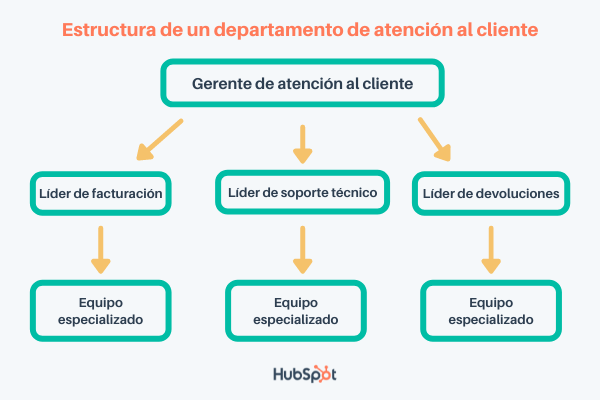
\includegraphics[width=.8\textwidth]{./Figures/atencionclienteestructura.png}
	\caption{Organigrama de un área de atención al cliente\protect\footnotemark.}
	\label{fig:atencionestructura}
\end{figure}

\footnotetext{Imagen tomada de \url{https://blog.hubspot.es/service/que-es-atencion-al-cliente}}

\subsection{El proceso de atención al cliente}

El proceso de atención al cliente consiste en una serie de pasos que se realizan para atender los reclamos y/o consultas que recibe la empresa \citep{WEBSITE:7}.

A continuación se describen los pasos principales de un proceso de atención típico \citep{WEBSITE:8}.

\begin{itemize}

\item Contacto y captura de la demanda del cliente: en esta etapa se recibe el mensaje del cliente por cualquiera de los canales establecidos y se procede a registrarlo en el sistema.
\item Análisis y clasificación: se analiza la información recibida y se evalúa si es suficiente para proceder a la clasificación del caso. De lo contrario se vuelve a contactar al cliente para obtener más detalles.
\item Resolución: en esta etapa se busca dar una respuesta a la consulta o reclamo del cliente. En algunos casos puede involucrar varios equipos o personas, por lo que su duración es variable.
\item Cierre: en esta etapa se presenta la solución al cliente y se le comunican los próximos pasos si los hubiera.

\end{itemize}

%----------------------------------------------------------------------------------------

\section{Motivación}

Hoy en día al cliente se le hace muy fácil pasar a la competencia en caso de que la empresa no pueda cumplir con sus expectativas. Una mala \textit{CX (Customer Experience)} puede generar un efecto de bola de nieve, ya que los usuarios que hayan tenido una mala experiencia, son mas propensos a comunicarlo con sus conocidos haciendo que la empresa no sólo pierda un cliente sino que ademas, se le dificulte expandir su mercado \citep{WEBSITE:9}.

Según informes de \textit{CX Trends} \citep{cxtrends}\citep{WEBSITE:4}\citep{WEBSITE:10} y de Esteban Kolsky \citep{WEBSITE:11}:

\begin{itemize}
\item El 70\% de los consumidores gastará más en una empresa que ofrezca una buena \textit{CX}.
\item El 50\% de los clientes se pasaría a la competencia después de haber tenido tan solo una mala experiencia. Este valor sube a un 80\% si se les pregunta si hubieran tenido dos o más malas experiencias.
\item El 72\% de los clientes compartiría una experiencia positiva con 6 o más personas.
\item El 13\% de los clientes compartiría su experiencia con 15 o más personas si no está satisfecho.
\item Sólo el 3.85\% de los clientes insatisfechos se lo comunican a la empresa.
\end{itemize}

Estos números muestran que la ausencia de quejas no es un signo de satisfacción. Por el contrario, es probable que los clientes hayan abandonado la empresa y estén compartiendo su insatisfacción con otras personas. También muestran la importancia de mantenerlos satisfechos, ya que son propensos a compartirlo.

Más aún, entre las principales razones de una mala atención al cliente se encuentran tener tiempos de espera demasiado largos \citep{WEBSITE:12} y tener muchas derivaciones internas \citep{WEBSITE:13}.

De todo esto se deduce que resulta muy importante que los procesos del área se realicen de forma eficiente. La utilización de modelos de IA para automatizar el proceso de clasificación de reclamos y consultas, ayuda a la empresa a responder a sus clientes con tiempos de respuesta menores y permite disponer de más analistas en la etapa de resolución y cierre. De esta manera, se genera una imagen positiva de la empresa que facilita la fidelización de clientes existentes y aumenta la incorporación de los nuevos.

%----------------------------------------------------------------------------------------

\section{Estado del arte}

El PNL (Procesamiento del lenguaje natural) es un subcampo de la inteligencia artificial que busca enseñar a un programa informático a comprender, interpretar y generar texto en lenguaje humano. A principios del siglo XXI, el PNL experimentó un crecimiento significativo gracias a la aplicación de algoritmos de aprendizaje profundo y la disponibilidad de grandes corpus de texto \citep{WEBSITE:14}. 

En 2003, Yoshua Bengio et al. entrenan la primer red neuronal orientada al lenguaje, utilizando vectores para representar palabras. Llamarían a este proceso "aprender una representación distribuida para cada palabra" \citep{ARTICLE:1}.

En 2008 Ronan Collobert y Jason Weston introducen el concepto de \textit{Word Embeddings} como una herramienta potente para tareas de PNL. Se distinguirían de sus antecesores mencionando que su objetivo era predecir la relevancia de una palabra dada la parte previa y posterior de la oración, a diferencia de el trabajo previo que buscaba predecir la probabilidad de una palabra dada la parte previa de una oración.

En 2013, Tomas Mikolov et al. publican su artículo dónde detallan las arquitecturas \textit{CBOW} y \textit{Skip-Gram}. Además liberan el primer modelo pre-entrenado llamado \textit{Word2Vec} (basado en \textit{Skip-Gram}) popularizando el uso de los \textit{Word Embeddings} \citep{ARTICLE:3}.

Posteriormente, en 2014, Pennington et al. publicarían \textit{GloVe} como otro método de generación de \textit{Word Embeddings} que utiliza una probabilidad de co-ocurrencia \citep{ARTICLE:4}. Con esta técnica, si dos palabras co-existen muchas veces, ambas palabras tienen una probabilidad alta de tener un mismo significado.

Los \textit{Word Embeddings} se convirtieron en la herramienta principal dentro del PNL. Capturan el significado de una palabra y la traducen a una representación numérica que puede ser usada como entrada para las redes neuronales.

El avance del aprendizaje profundo, permitió a los investigadores desarrollar arquitecturas de redes neuronales más avanzadas y eficientes. 

Sin embargo, no fue hasta 2017, cuando Vaswani et. al publican la utilización de un mecanismo de atención para desarrollar una nueva arquitectura que ellos llamarían \textit{Transformers} que se marca un verdadero hito \citep{ARTICLE:5}. Las redes más usadas hoy en día como \textit{BERT} o \textit{ChatGPT} están basados en esta mejora.

El mecanismo de atención le sirve a la red para saber a que parte de la oración de entrada le tiene que prestar más atención para cada elemento de la salida. Este enfoque tiene la limitante de que cada secuencia debe ser procesada de a una a la vez.

Los \textit{Transformers} vienen a solucionar este problema con un mecanismo de "atención propia" que permite una mayor paralelización.


%----------------------------------------------------------------------------------------

\section{Objetivos y alcance}



\chapter{Introducción específica} % Main chapter title

\label{Chapter2}

%----------------------------------------------------------------------------------------
%	SECTION 1
%----------------------------------------------------------------------------------------
En este capítulo se enumeran los requisitos que la solución debe cumplir y luego se describen principalmente las herramientas utilizadas durante el desarrollo para el entrenamiento y despliegue de los modelos para satisfacerlos.

\section{Requerimientos}

En esta sección se detallan los requerimientos funcionales y las restricciones de implementación del trabajo.


\begin{enumerate}
	\item Requerimientos funcionales
	\begin{enumerate}
		\item El sistema debe poder detectar la categoría de un reclamo escrito en lenguaje natural.
		\item El sistema debe poder detectar la categoría de una consulta escrita en lenguaje natural.
		\item El usuario debe poder utilizar los resultados de la clasificación desde una base de datos.
		\item El proceso debe ser capaz de interpretar errores de ortografía.
		\item El proceso debe ser capaz de adaptarse a distinta cantidad de palabras en el mensaje.
		\item La solución debe ejecutarse en forma \textit{batch}, corriendo diariamente y tomando los casos del día anterior.
	\end{enumerate}
	\item Requerimientos no funcionales
	\begin{enumerate}
		\item El sistema debe estar desarrollado en lenguaje Python.
		\item El código debe ser versionado con Git.
		\item La solución debe estar desplegada sobre infraestructura de Google Cloud Platform.
		\item La salida de los modelos debe ser almacenada en BigQuery.
		\item El proceso debe ser ejecutado a través del orquestador Apache Airflow.
	\end{enumerate}
	\item Requerimientos de testing
	\begin{enumerate}
		\item Se deben generar métricas de desempeño de los modelos con el dataset de entrenamiento y de prueba.
	\end{enumerate}
	\item Requerimientos de documentación
	\begin{enumerate}
		\item Se debe confeccionar un documento con el diseño de la arquitectura de alto nivel.
		\item Se debe confeccionar un documento con el diseño de los modelos de IA.
		\item Se debe confeccionar un documento que especifique los datos que consumen los modelos y su origen.
	\end{enumerate}
\end{enumerate}



\section{Preprocesamiento del texto}

En esta sección se introducen las herramientas utilizadas para realizar la limpieza y preparación del texto que sirvió tanto para la parte de entrenamiento como para la parte de predicción en el despliegue.

\subsection{Natural Language Toolkit}

NLTK \textit{(Natural Language Toolkit)} es una librería de Python para preprocesar texto. Es una de las herramientas principales del mercado y entre otras cosas permite:
\begin{itemize}
\item Realizar la ``tokenización'' o segmentación del texto.
\item Remover \textit{stopwords} o palabras vacías.
\item Aplicar \textit{stemming} sobre las palabras.
\item Realizar ``lematización'' sobre las palabras.
\item Etiquetar cada término en una oración según sea sustantivo, verbo, adjetivo, preposición, etc.
\end{itemize}

A continuación se profundizará en las funcionalidades de esta librería que se usaron para este trabajo.

\subsubsection{Segmentación}

La segmentación consiste en separar un documento en términos individuales. Estos términos se llaman \textit{tokens} y es la unidad mínima de análisis de texto. Dependiendo de la tarea en cuestión, un \textit{token} puede ser una palabra, una sílaba o incluso un solo caracter.

Esta etapa es importante porque sirve como base para las etapas posteriores del preprocesamiento del texto.

\subsubsection{Remoción de palabras vacías}

Las \textit{stopwords} o palabras vacías son palabras que son muy comunes en el idioma español y están destinadas a aparecer en todas las oraciones, sin importar el tema al que hagan referencia \citep{WEBSITE:16}, por ejemplo: ``en'', ``este'', ``el'', ``las''.

Eliminar palabras comunes permite eliminar palabras con poco valor discriminativo entre textos (o categorías de reclamos). Además reduce el volumen de datos a procesar.

\subsubsection{Derivación}

El \textit{stemming} o derivación o poda consiste en recortar las palabras para reducirlas a una base común. Es decir, devuelve el tallo de una palabra, que no necesariamente es igual a la raíz morfológica de la palabra. Por ejemplo, para la palabra ``comienza'' su derivación será ``comienz'' y para ``peces'' será ``pec''.

La idea detrás de esta técnica es tratar de agrupar las palabras similares, reduciendo la cantidad de palabras únicas en un \textit{dataset}.

\subsection{Scikit-Learn}

Scikit-Learn es una librería de Python para \textit{Machine Learning} que cuenta con una variedad de algoritmos y modelos para clasificación y regresión. Además cuenta con un conjunto de herramientas de extracción y generación de variables, tanto para datos numéricos como para texto.

A continuación se dará una explicación de los módulos usados de esta librería.

\subsubsection{Normalización de etiquetas}

La normalización de etiquetas o \textit{label encoding} consiste en codificar variables categóricas en valores numéricos que irán entre 0 y $n-1$ siendo $n$ la cantidad de categorías. Es decir, asigna un número único a cada categoría. De esta forma, al entrenar los modelos de IA se puede pasar la variable \textit{target} en formato numérico. 

Otra utilidad muy importante de la versión que trae Scikit-Learn es la posibilidad de realizar la transformación inversa. Esto resulta muy útil para determinar el texto de la variable numérica que predice el modelo.

En la figura \ref{fig:labelencoding} se puede ver un ejemplo de la transformación.

\begin{figure}[htbp]
	\centering
	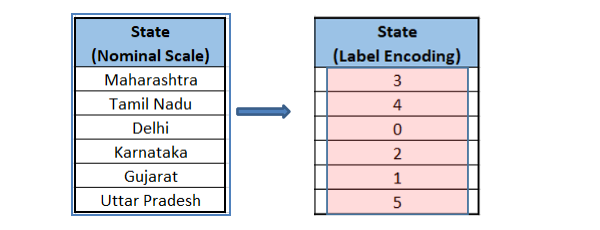
\includegraphics[width=.8\textwidth]{./Figures/labelencoding.png}
	\caption{Ejemplo de codificación realizado sobre una variable\protect\footnotemark.}
	\label{fig:labelencoding}
\end{figure}

\footnotetext{Imagen tomada de \url{https://www.mygreatlearning.com/blog/label-encoding-in-python/}}

\subsubsection{Vectorizador Term Frequency - Inverse Document Frequency}

La vectorización es una técnica de PNL que convierte una secuencia de \textit{tokens} (obtenidos previamente en la etapa de segmentación) a un vector numérico.

Hay distintas maneras de realizar este proceso, la elegida para este trabajo es la que se conoce como TF-IDF \textit{(Term Frequency - Inverse Document Frequency)}. Su objetivo es reflejar cuán importante es una palabra respecto al documento. \textit{Nota: Para este trabajo, la palabra documento representa un caso de reclamo o consulta de un cliente}. 

Tiene dos partes: el cálculo de TF y el cálculo de IDF.

TF calcula para cada documento del \textit{dataset}, la cantidad de veces que un \textit{token} aparece en él. Es decir, calcula la frecuencia de un \textit{token} en cada documento. Luego, ese número se divide por la cantidad de palabras que tenía ese documento. 
La fórmula para calcularla es la siguiente \citep{WEBSITE:17}
\begin{equation}
tf_{i,j}= \frac{n_{i,j}}{\sum_{_{k}}^{}n_{i,j}}
\end{equation}

IDF calcula la proporción de documentos del \textit{dataset} que poseen el \textit{token}. Es decir, divide la cantidad total de documentos sobre la cantidad de documentos con ese \textit{token}, y luego a ese resultado le aplica el logaritmo. Los términos raros tendrán un puntaje más alto. 
La siguiente ecuación muestra cómo se calcula:
\begin{equation}
idf(w) = log(\frac{N}{df_{i}})
\end{equation}
Finalmente, una vez obtenidos el TF y el IDF, lo que se hace es multiplicar ambos términos para cada \textit{token} en todos los documentos:
\begin{equation}
w_{i,j} = tf_{i,j} \times idf(w)
\end{equation}

\section{Modelos de inteligencia artificial utilizados}

En esta sección se presentan los modelos de IA utilizados.

\subsection{Complement Naive Bayes}

Los algoritmos de \textit{Naive Bayes} o Bayes ingenuo son muy utilizados para tareas de clasificación por su velocidad de cómputo. Son modelos probabilísticos que deben su nombre a la probabilidad condicional y el teorema de Bayes. Se les denomina ingenuos porque suponen una independencia entre variables, que muchas veces no es real \citep{WEBSITE:18}.

Para este trabajo se seleccionó particularmente el modelo CNB (\textit{Complement Naive Bayes}), que es una adaptación del MNB (\textit{Multinomial Naive Bayes}), pero que se adecúa mejor al desbalanceo entre clases. Por lo general, CNB supera a MNB en tareas de clasificación de texto \citep{ARTICLE:6}.

Lo que hace el algoritmo es calcular, para cada clase, la probabilidad de que un documento no le pertenezca. Luego, la clase del documento será la clase con menor probabilidad, ya que aquí se quiere minimizar la probabilidad de no pertenecer.

La fórmula de CNB es la siguiente \citep{WEBSITE:19}:
\begin{equation}
l(t) = \arg \min \sum_{i}^{}t_{i}w_{ci}
\end{equation}
donde $t_{i}$ es la cantidad de veces que aparece el \textit{token} $i$ en el documento y:
\begin{equation}
w_{ci} = \frac{\log{\widehat{\theta}_{ci}}}{\sum_{k}^{}|\log{\widehat{\theta}_{ck}}|}
\end{equation}
siendo:
\begin{equation}
\label{eq:tita}
\widehat{\theta}_{ci} = \frac{\alpha_{i} + \sum_{_{j:y_{j}\neq c}}^{}d_{ij}}{\alpha+\sum_{j:y_{j\neq c}}^{}\sum_{k}^{}d_{kj}}
\end{equation}
donde las sumatorias son sobre todos los documentos $j$ que no sean de la clase $c$ , $d_{ij}$ es la cantidad de veces que aparece el \textit{token} en el documento $j$, $\alpha_{i}$ es un hyperparámetro de suavizado (por lo general equivale a 1) y $\alpha = \sum_{i}^{}\alpha_{i}$.
\subsection{Representaciones de codificador bidireccional de transformadores}

BERT \textit{(Bidirectional Encoder Representations from Transformers)} es un modelo \textit{open source} de PNL desarrollado por Google en el año 2018. El modelo original fue entrenado con texto de Wikipedia y el \textit{dataset} BookCorpus de Google.

Inicialmente, dos modelos de BERT fueron presentados:
\begin{itemize}
	\item \textit{base}: con 12 capas, 12 cabezas de atención y 110 millones de parámetros.
	\item \textit{large}: con 24 capas, 16 cabezas de atención y 340 millones de parámetros.
\end{itemize}

Cada capa de BERT es un \textit{Transformer Encoder}. Cuando se habla de, por ejemplo, 12 capas, son 12 de esos codificadores apilados uno encima de otro. Los datos de entrada son consumidos por la primer capa, y van pasando por cada una hasta llegar a la última. Como salida, habrá un \textit{embedding} donde cada posición del \textit{token} tendrá un vector de 768 posiciones para BERT \textit{base} y 1024 para BERT \textit{large} \citep{WEBSITE:20}.

La innovación introducida por BERT es aplicar dos técnicas en la etapa de entrenamiento: MLM \textit{(Masked Language Model)} y NSP \textit{(Next Sentence Prediction)}. 

MLM consiste en dar a BERT una secuencia para que optimice sus pesos internos y produzca la misma secuencia. Sin embargo, previamente a dar a BERT la secuencia, se enmascaran ciertos \textit{tokens} para que BERT los tenga que ``adivinar''. La implicancia de esta técnica es que BERT termina aprendiendo del contexto de la oración para predecirlos.

Para lograr esto, BERT se apoya en un mecanismo de atención propia o \textit{self-attention} posibilitado por los \textit{Transformers} bidireccionales en el núcleo del diseño de BERT. Esto es importante ya que el significado de una palabra puede cambiar a medida que se desarrolla una oración. Cuantas más palabras haya en cada oración o frase, más ambigua se  vuelve la palabra en cuestión. BERT se encarga de esta ambigüedad leyendo una oración bidireccionalmente, teniendo en cuenta el efecto de todas las palabras en la oración y no sólo las que la preceden \citep{WEBSITE:21}.

En la figura \ref{fig:selfattention} se puede ver cómo para una palabra, el modelo de IA hace una ponderación de la importancia del resto de las palabras en esa oración.

\begin{figure}[htbp]
	\centering
	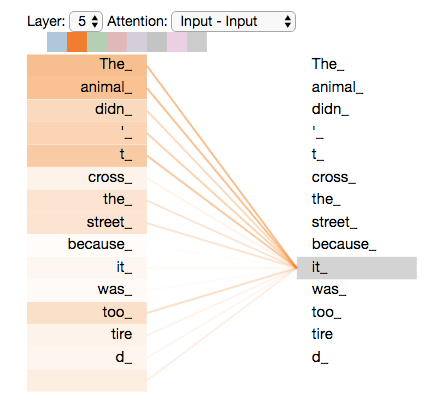
\includegraphics[width=.6\textwidth]{./Figures/selfattention.png}
	\caption{Ejemplo de funcionamiento del mecanismo de atención propia\protect\footnotemark.}
	\label{fig:selfattention}
\end{figure}

\footnotetext{Imagen tomada de \url{https://towardsdatascience.com/understand-self-attention-in-bert-intuitively-cd480cbff30b}}

NSP, por otro lado, es otro mecanismo en donde el modelo recibe oraciones de a pares como entrada y aprende a predecir si la segunda oración en el par es subsecuente de la primera. Durante el entrenamiento, la mitad de los datos son pares de oraciones subsecuentes y en la otra mitad la segunda oración es seleccionada de manera aleatoria.

Para saber distinguir cuándo comienza la primer oración y cuándo la segunda, la entrada es procesada de la siguiente forma:

\begin{enumerate}
	\item Un \textit{token} ``[CLS]'' se inserta al comienzo de la primer oración y un \textit{token} ``[SEP]'' es insertado al final de las dos oraciones.
	\item Se agrega un \textit{embedding} que indica para cada \textit{token} si corresponde con la oración A o B.
	\item Se agrega un \textit{embedding} posicional que indica para cada \textit{token} su posición en la secuencia.
\end{enumerate}

En la figura \ref{fig:bertinput} se puede ver cómo se combinan estas dos técnicas cuando se entrena BERT.

\begin{figure}[htbp]
	\centering
	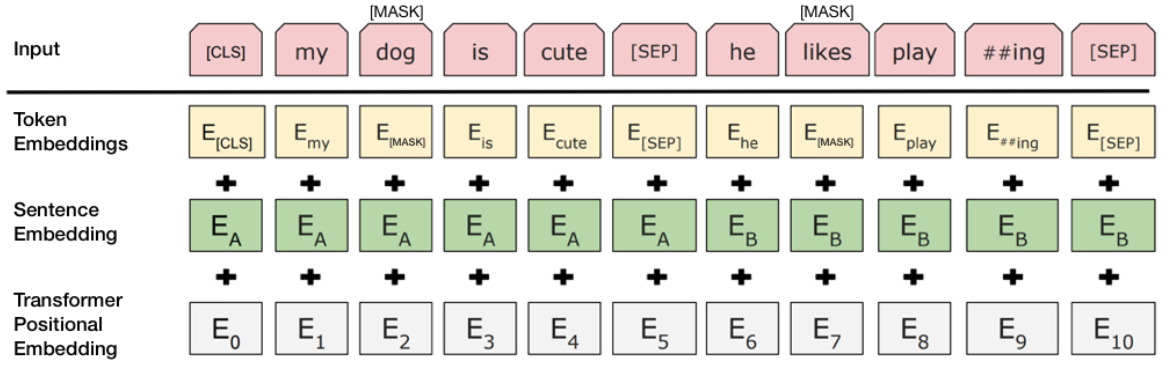
\includegraphics[width=.8\textwidth]{./Figures/bertinput.png}
	\caption{Ejemplo de entrada de datos a BERT con MLM y NSP combinados\protect\footnotemark.}
	\label{fig:bertinput}
\end{figure}

\footnotetext{Imagen tomada de \url{https://towardsdatascience.com/bert-explained-state-of-the-art-language-model-for-nlp-f8b21a9b6270}}

En la primera fila se observa cómo fueron separadas las dos oraciones. Luego en el \textit{embedding} amarillo, se observa cómo algunos \textit{tokens} son enmascarados para que luego la red los tenga que predecir. En el tercera, en verde, se observa la asignación de cada \textit{token} a la oración A o B y por último, se observa un \textit{embedding} con el orden de cada \textit{token}.

\section{Herramientas de software utilizadas}

En esta sección se presentan las herramientas que se utilizaron tanto para la fase de entrenamiento como para el despliegue de los modelos.

\subsection{Python}

Python es un lenguaje de programación utilizado principalmente para desarrollo de aplicaciones y \textit{machine learning}. Entre sus características se destaca que es orientado a objetos, multiplataforma e interpretado y su tipado es dinámico y fuerte \citep{WEBSITE:32}.

\subsection{GitHub}

GitHub es un servicio web donde los usuarios pueden alojar repositorios con Git como sistema de control de versiones. Este sistema permite gestionar y rastrear cambios en el código a través del tiempo, ayudando a los equipos de desarrolladores a trabajar en proyectos de manera colaborativa \citep{WEBSITE:33}.

Por otro lado, tiene una plataforma de integración y despliegue continúo llamada GitHub Actions. Esta plataforma permite crear y configurar la ejecución de flujos de trabajo o \textit{workflows} cuando un evento sucede en el repositorio \citep{WEBSITE:37}.

\subsection{BigQuery}
\label{cap2-bq}

BigQuery es un servicio \textit{serverless} de \textit{Data Warehouse} de GCP (Google Cloud Platform). Los datos se guardan en colecciones de tablas, que a su vez, se agrupan en \textit{datasets}. Cada columna de las tablas se almacena por separado, por eso se dice que BigQuery es una base de datos columnar \citep{WEBSITE:30}.

El acceso a los datos se hace a través del lenguaje SQL. Los recursos que se necesiten para ejecutar una consulta se calculan dinámicamente en base a sus características y también en cómo esté configurada la tabla.

\subsection{Vertex AI workbench}

Vertex es un entorno de desarrollo especializado para ciencia de datos. Permite disponibilizar un \textit{Jupyter notebook} que se integra con BigQuery y Google Cloud Storage para la lectura de datos y con GitHub para la sincronización de código. Además posee instancias con distintas configuraciones de CPU y GPU \citep{WEBSITE:34}. 

\subsection{Docker}

Docker es una herramienta que empaqueta \textit{software} en unidades llamadas contenedores, que incluyen todas las dependencias para que el programa se ejecute: ejecutables, archivos de configuración, bibliotecas, etc. Funciona de manera similar a una máquina virtual, solo que además de virtualizar el hardware también virtualiza el sistema operativo \citep{WEBSITE:35}.

La principal ventaja que otorga el uso de Docker es que asegura que el contenedor se pueda ejecutar de manera fiable en cualquier plataforma compatible, como Kubernetes.

\subsection{Artifact registry}

Artifact Registry permite almacenar y administrar imágenes de Docker. Posibilita armar un \textit{pipeline} de integración y despliegue continuo al permitir cargar una imagen de Docker para que pueda ser consumida desde las distintas plataformas de orquestación de contenedores \citep{WEBSITE:36}.

\subsection{Cloud Composer y Apache Airflow}

Cloud Composer es un servicio de organización de flujos de trabajo administrado por Google. Está basado en el proyecto \textit{open source} Apache Airflow \citep{WEBSITE:31}. 

Un flujo de trabajo representa una serie de tareas para trabajar con datos. Estos flujos son creados mediante grafos acíclicos dirigidos o DAGs \textit{(Directed Acyclic Graphs)}. Los DAGs se crean con código en Python que especifica su estructura. 
\chapter{Diseño e implementación} % Main chapter title

\label{Chapter3} % Change X to a consecutive number; for referencing this chapter elsewhere, use \ref{ChapterX}

\definecolor{mygreen}{rgb}{0,0.6,0}
\definecolor{mygray}{rgb}{0.5,0.5,0.5}
\definecolor{mymauve}{rgb}{0.58,0,0.82}

%%%%%%%%%%%%%%%%%%%%%%%%%%%%%%%%%%%%%%%%%%%%%%%%%%%%%%%%%%%%%%%%%%%%%%%%%%%%%
% parámetros para configurar el formato del código en los entornos lstlisting
%%%%%%%%%%%%%%%%%%%%%%%%%%%%%%%%%%%%%%%%%%%%%%%%%%%%%%%%%%%%%%%%%%%%%%%%%%%%%
\lstset{ %
  backgroundcolor=\color{white},   % choose the background color; you must add \usepackage{color} or \usepackage{xcolor}
  basicstyle=\footnotesize,        % the size of the fonts that are used for the code
  breakatwhitespace=false,         % sets if automatic breaks should only happen at whitespace
  breaklines=true,                 % sets automatic line breaking
  captionpos=b,                    % sets the caption-position to bottom
  commentstyle=\color{mygreen},    % comment style
  deletekeywords={...},            % if you want to delete keywords from the given language
  %escapeinside={\%*}{*)},          % if you want to add LaTeX within your code
  %extendedchars=true,              % lets you use non-ASCII characters; for 8-bits encodings only, does not work with UTF-8
  %frame=single,	                % adds a frame around the code
  keepspaces=true,                 % keeps spaces in text, useful for keeping indentation of code (possibly needs columns=flexible)
  keywordstyle=\color{blue},       % keyword style
  language=[ANSI]C,                % the language of the code
  %otherkeywords={*,...},           % if you want to add more keywords to the set
  numbers=left,                    % where to put the line-numbers; possible values are (none, left, right)
  numbersep=5pt,                   % how far the line-numbers are from the code
  numberstyle=\tiny\color{mygray}, % the style that is used for the line-numbers
  rulecolor=\color{black},         % if not set, the frame-color may be changed on line-breaks within not-black text (e.g. comments (green here))
  showspaces=false,                % show spaces everywhere adding particular underscores; it overrides 'showstringspaces'
  showstringspaces=false,          % underline spaces within strings only
  showtabs=false,                  % show tabs within strings adding particular underscores
  stepnumber=1,                    % the step between two line-numbers. If it's 1, each line will be numbered
  stringstyle=\color{mymauve},     % string literal style
  tabsize=2,	                   % sets default tabsize to 2 spaces
  title=\lstname,                  % show the filename of files included with \lstinputlisting; also try caption instead of title
  morecomment=[s]{/*}{*/}
}


En este capítulo se describe cómo se han utilizado las herramientas mencionadas en el capítulo \ref{Chapter2} y sus integraciones. Se presenta la arquitectura de alto nivel completa y luego se describe detalladamente desde el consumo de datos hasta la salida del proceso y su almacenamiento.


\section{Arquitectura del sistema}

En la figura \ref{fig:arqsistema} se puede observar la arquitectura de alto nivel que integra las herramientas utilizadas en la fase de entrenamiento y evaluación de los modelos de IA con las herramientas utilizadas para el despliegue.

\begin{figure}[htbp]
	\centering
	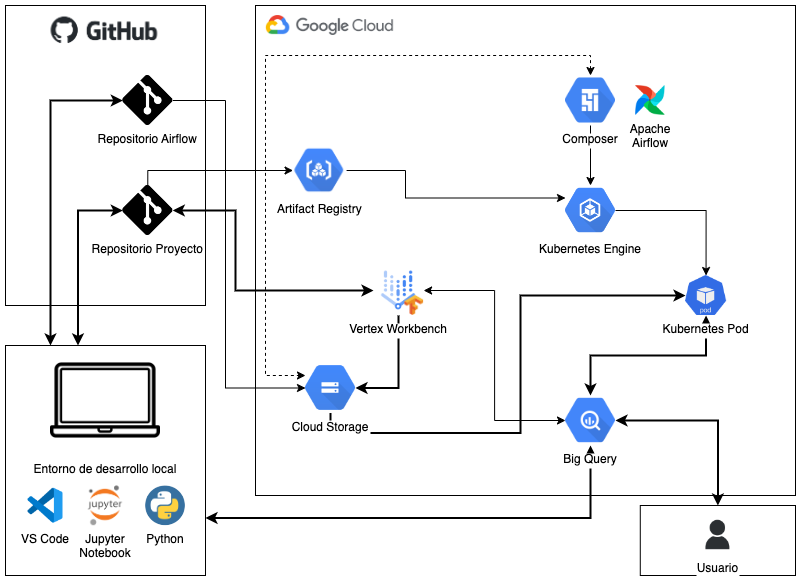
\includegraphics[width=1\textwidth]{./Figures/arq-sistema.png}
	\caption{Diagrama de la arquitectura de alto nivel.}
	\label{fig:arqsistema}
\end{figure}

La mayor parte del desarrollo se realizó en una computadora local, que contaba con un intérprete de Python y Visual Studio Code con Jupyter para la escritura de código. Estos archivos se sincronizaban contra un repositorio de GitHub.

Los datos para realizar el entrenamiento de los modelos de IA fueron tomados del \textit{data warehouse} BigQuery utilizando consultas SQL y bibliotecas de Google para Python para manejar su ejecución.

Estos datos son llevados a BigQuery por un proceso ajeno a este desarrollo, que se encarga de sincronizar la base de Salesforce hacia el \textit{data warehouse} diariamente. Particularmente, hay una tabla que contiene los reclamos y consultas de los usuarios, con su identificador de caso, fecha de creación y estado.

En las ocasiones en las que fue necesario un mayor poder de cómputo a través del uso de una placa de vídeo dedicada, se utilizó una instancia de Vertex AI Workbench en la nube de Google. Por lo general, estas situaciones se dieron al momento de realizar distintas pruebas con las redes neuronales BERT. Los modelos eran luego exportados al almacenamiento de la nube llamado Cloud Storage en formato ``Pickle'' o ``HDF5'' \textit{(Hierarchical Data Format 5)}.

El repositorio del proyecto cuenta con un Workflow de GitHub Action que se corre manualmente y genera una imagen de Docker, incluyendo bibliotecas y librerías necesarias, archivos de código y de configuración. Esta imagen de Docker es enviada al Artifact Registry de la nube de Google y almacenada allí.

Por otro lado, se trabajó en otro repositorio separado, que es único para manejar todos los flujos de trabajo de Apache Airflow que tiene el área de \textit{machine learning}. Este repositorio es exclusivo para la etapa de despliegue, y se agregó el DAG que administra el proceso de predicción.

El repositorio de Airflow cuenta con un Workflow de GitHub Action que sincroniza el código de los DAGs contra un Cloud Storage que está conectado a la instancia del orquestador. Airflow periódicamente controla si hay un flujo de trabajo nuevo y cuando lo detecta, lo carga.

Al momento de ejecutar el proceso, Airflow utiliza un operador dentro del DAG para conectarse con la plataforma de Kubernetes en instancia un Pod. Este Pod ejecuta los archivos de código del contenedor que se empaquetaron en la imagen de Docker cargada previamente en el Artifact Registry.

Al finalizar, se guardan los resultados de las predicciones en una tabla en BigQuery y el Pod es eliminado de Kubernetes. Los datos quedan disponibles en la base para que cualquier usuario con los suficientes permisos pueda consumirlos ejecutando una consulta a la base.

\section{Extracción y preprocesamiento del texto}

En esta sección se describen en detalle los pasos realizados para obtener los datos crudos y aplicarles un preprocesamiento para poder usarlos de entrada en el posterior entrenamiento de los modelos de IA.

\subsection{Extracción de datos de BigQuery}

Inicialmente se realizó un relevamiento de las tablas existentes, y en particular se encontró una tabla que contenía información de los reclamos y consultas. 

Las columnas de interés de esa tabla fueron:
\begin{itemize}
	\item El identificador del caso.
	\item El número del caso.
	\item La categoría L2 (de segundo nivel).
	\item La categoría L3 (de tercer nivel).
	\item El estado del caso.
	\item La descripción: el contenido del mensaje que escribió el usuario.
	\item La fecha de creación.
	\item La fecha de cierre.
\end{itemize}

Para la fase de entrenamiento, se limitó la extracción de casos a los que tenían fecha de creación entre enero de 2021 y diciembre de 2022. Además, su estado debía ser ``Resuelto'' o ``Cerrado''. Sin embargo, por la poca cantidad de datos que había para algunos clasificadores L2, fue necesario realizar consultas adicionales para tomar casos de 2023. Una vez obtenidos los datos, se guardaron en archivos ``Parquet'' para su posterior uso con la librería Pandas para Python.

Por otro lado, el área de atención al cliente maneja un archivo CSV \textit{(comma-separated values)} con la jerarquía de casos L1, L2 y L3. Es decir, para cada L1, qué casos L2 le corresponden, y para cada uno de esos L2, qué casos L3 le corresponden. Las categorías L3 fueron ignoradas para este trabajo, por lo que se hará foco en las primeras dos.

En total, se encontraron 15 categorías L1 y 122 categorías L2. Luego de una reunión con el área de atención al cliente para un mejor entendimiento de cada una, se descartó una categoría especial. Luego de este refinamiento quedaron 14 L1 y 117 L2.

En la figura \ref{fig:catl2porl1} se puede observar para cada categoría L1 cuántas subcategorías L2 contiene.

\begin{figure}[htbp]
	\centering
	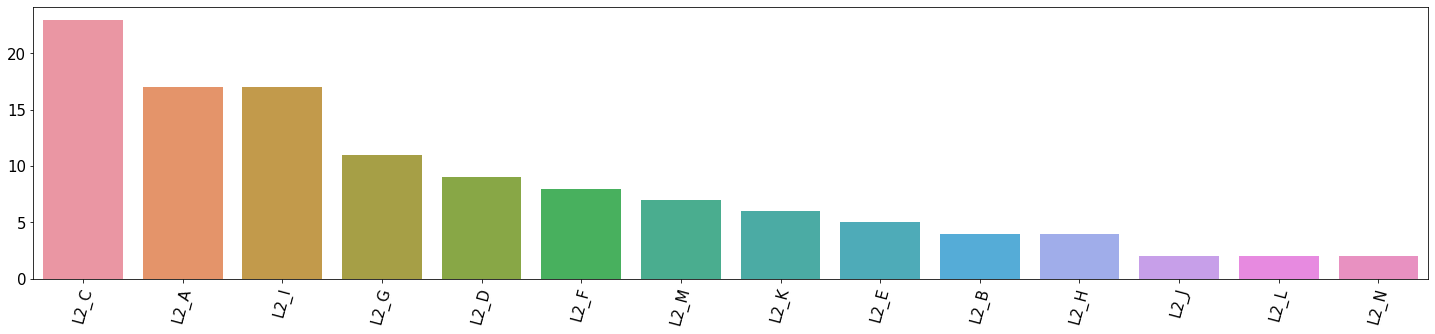
\includegraphics[width=1\textwidth]{./Figures/catl2porl1.png}
	\caption{Cantidad de categorías L2 para cada L1.}
	\label{fig:catl2porl1}
\end{figure}

Para trabajar en la fase de preprocesamiento, se combinó el archivo de los casos con el archivo que contenía la jerarquía de categorías, obteniendo así la L1 de cada reclamo y consulta.

\subsection{\textit{Pipeline} de preprocesamiento}

El preprocesamiento es una de las tareas más importantes en PNL. Los datos en crudo pueden contener información que no es relevante para la tarea en cuestión, que se debe eliminar. Por otro lado, muchos modelos de IA requieren un formateo previo de los datos para poder consumirlos.

En la figura \ref{fig:pipeline-texto} se detallan los pasos realizados para ``limpiar'' el texto.

\begin{figure}[htbp]
	\centering
	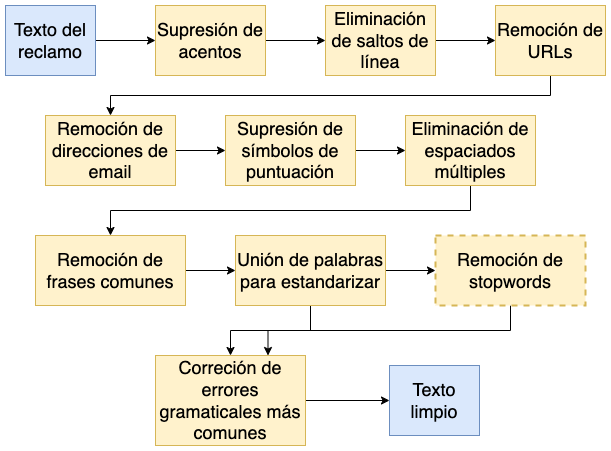
\includegraphics[width=.7\textwidth]{./Figures/pipeline-texto.png}
	\caption{Diagrama del procesamiento del texto crudo.}
	\label{fig:pipeline-texto}
\end{figure}

El proceso comienza con el texto original del reclamo tal cual quedó guardado en la base. Luego se le aplican las siguientes acciones:
\begin{enumerate}
	\item Se suprimen los acentos de las palabras (si los hubiera) utilizando una expresión regular.
	\item Se eliminan los saltos de línea.
	\item Se sacan URLs en el mesaje en caso de que hubiese hipervínculos.
	\item Se sacan direcciones de \textit{email}. Estos por lo general aparecen cuando el reclamo se hace a través de ese medio.
	\item Se suprimen signos de puntuación utilizando otra expresión regular.
	\item Se eliminan espacios múltiples para normalizar en un espacio entre dos palabras.
	\item Se remueven frases que se repiten en muchos reclamos: algunos casos quedan registrados en la base con la respuesta por parte de la empresa. Estos mensajes tienen una plantilla de base con frases que luego se repiten entre casos.
	\item Se unen palabras con un significado específico: por ejemplo ``pedidos ya'' se deja como ``pedidosya'' porque hace referencia a una empresa.
	\item Para el caso de los modelos de CNB entrenados, se aplicó un paso extra para eliminar \textit{stopwords}.
	\item Por último se realizó un análisis con los datos de entrenamiento para ver los errores gramaticales más comunes utilizando la librería PyEnchant para Python. De esto se obtuvo un listado con los errores más comunes y un mapeo a su versión correcta. En este paso se aplica la corrección sobre ese listado de palabras.
\end{enumerate}

Una vez obtenido el texto limpio, se procede a pasarlo a un vector numérico para que sea intepretado por los modelos de IA. Se distinguen dos formas de hacerlo, dependiendo de si se usa el modelo de CNB o el de BERT.

\subsubsection{Codificación para CNB}

En la figura \ref{fig:pipeline-baseline} se explica el proceso para obtener los vectores numéricos para entrenar el modelo de CNB. Al texto limpio se le aplica un paso de segmentación para obtener los \textit{tokens} que luego serán vectorizados utilizando el método TF-IDF. Por otro lado, a la variable objetivo que también esta en formato de texto, se le aplica el proceso de \textit{label encoding} para obtener una variable numérica. 

\begin{figure}[htbp]
	\centering
	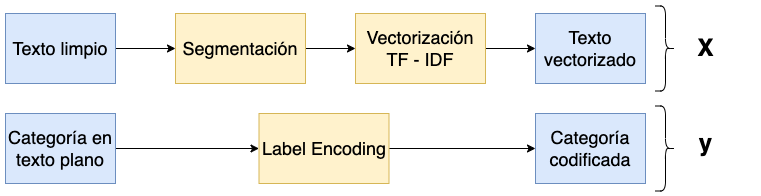
\includegraphics[width=.7\textwidth]{./Figures/pipeline-baseline.png}
	\caption{Diagrama de codificación para CNB.}
	\label{fig:pipeline-baseline}
\end{figure}

\subsubsection{Codificación para BERT}

En la figura \ref{fig:pipeline-bert} se puede ver el proceso para el caso de BERT. Se puede notar que es un poco mas largo que el de CNB.

\begin{figure}[htbp]
	\centering
	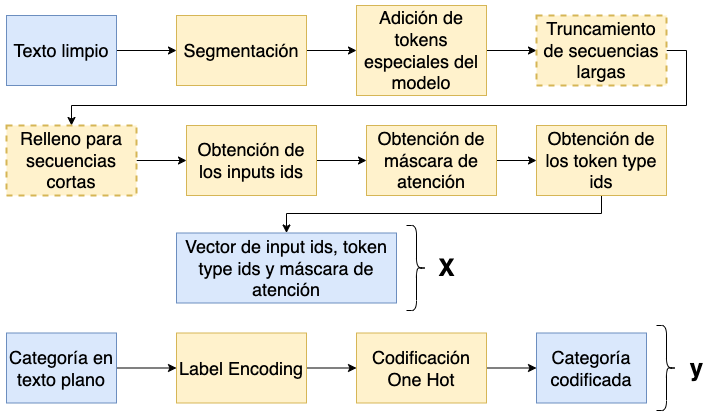
\includegraphics[width=.7\textwidth]{./Figures/pipeline-bert.png}
	\caption{Diagrama de codificación para BERT.}
	\label{fig:pipeline-bert}
\end{figure}

El algoritmo de segmentación de BERT se llama \textit{WordPiece} y tiene la particularidad de que no sólo segmenta por palabras sino que también lo hace por subpalabras y por caracteres. Arranca segmentando por todos los caracteres del vocabulario con el que fue entrenado y luego los va uniendo en pares. 

Utiliza la siguiente fórmula para computar los puntajes de los pares de \textit{tokens} a unir:
\begin{equation}
puntaje = \frac{\text{frecuencia del par}}{\text{frecuencia del primer elemento}\times \text{frecuencia del segundo elemento}}
\end{equation}
Luego une los pares con mayor puntaje y re-calcula para todos los \textit{tokens} resultantes. Este proceso es repetido hasta alcanzar un umbral para el puntaje o hasta alcanzar un límite de \textit{tokens}.

El vocabulario del modelo pre-entrenado de BERT que se utilizó está compuesto por 977 \textit{tokens} reservados del estilo ``[MASK]'' o ``[PAD]'' por ejemplo y luego por \textit{tokens} de caracteres individuales, subpalabras y palabras. \citep{WEBSITE:22}

En la figura \ref{fig:segmentacion-bert} podemos ver un ejemplo de cómo es segmentada una oración.

\begin{figure}[htbp]
	\centering
	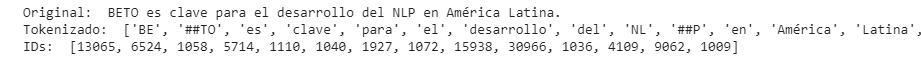
\includegraphics[width=1\textwidth]{./Figures/cap3-segmentacion.png}
	\caption{Ejemplo de segmentación \textit{WordPiece}\protect\footnotemark.}
	\label{fig:segmentacion-bert}
\end{figure}

\footnotetext{Imagen tomada de \url{https://espejel.substack.com/p/beto-bert-01-importacion-y-tokenizing}}

Luego de hacer la segmentación de cada frase, se hace un truncamiento de las secuencias largas a un máximo preestablecido y se realiza un relleno a las secuencias cortas con un \textit{token} especial hasta ocupar ese mismo máximo.

Los siguientes pasos son obtener los \textit{input ids} que son los identificadores de los \textit{tokens}, obtener la máscara de atención que marca qué \textit{tokens} la red debe mirar y por último obtener los \textit{token type ids} que marcan a qué secuencia pertenece cada \textit{token} (recordar que BERT se entrena de a pares de secuencia).

Por otro lado, la codificación de la variable objetivo es igual que en CNB solo que a la variable numérica obtenida se le aplica una codificación \textit{one hot} adicional.

\section{Entrenamiento de los modelos}

En esta sección se describe en detalle: los análisis exploratorios realizados sobre los datos, cómo fue concebida la solución de los modelos de IA, y las técnicas utilizadas para entrenar los modelos.

\subsection{Análisis exploratorio}

En la figura \ref{fig:cap3-distribucion} se observa la proporción de casos de cada categoría L1 sobre el total. Se puede ver que hay una que tiene casi el 50\%.

\begin{figure}[htb]
	\centering
	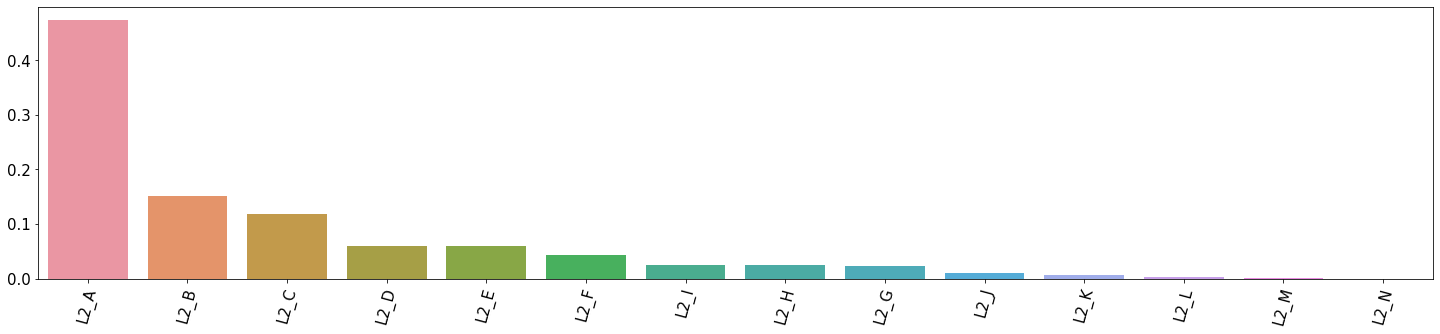
\includegraphics[width=1\textwidth]{./Figures/cap3-distribucion.png}
	\caption{Proporción de casos.}
	\label{fig:cap3-distribucion}
\end{figure}

También se realizó un análisis de las longitudes de los textos. En promedio, la cantidad de palabras en los mensajes fue de 78 previo a aplicar preprocesamiento, 71 aplicando una parte (se dejan las \textit{stopwords}) y 44 cuando se aplicó el preprocesamiento completo.

En la figura \ref{fig:cap3-longitudes} podemos observar la longitud promedio para cada categoría. En cada barra se puede ver la longitud del texto sin preprocesamiento, con preprocesamiento dejando \textit{stopwords} y también removiéndolas. Hay dos categorías cuya longitud promedio es particularmente elevada.

\begin{figure}[htbp]
	\centering
	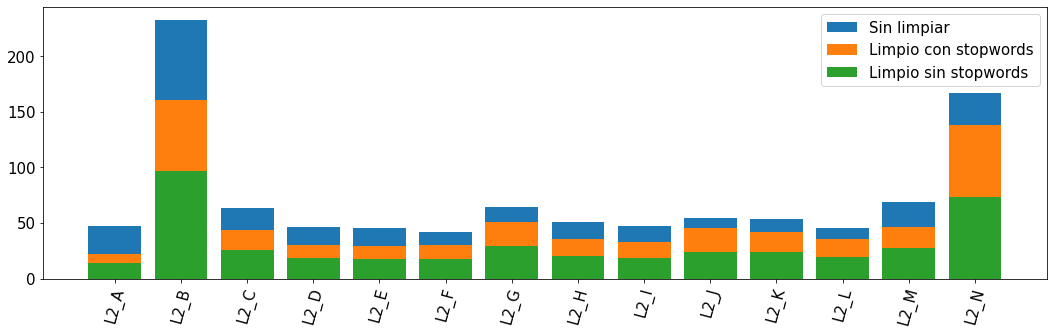
\includegraphics[width=1\textwidth]{./Figures/cap3-longitudes.png}
	\caption{Longitud de los mensajes.}
	\label{fig:cap3-longitudes}
\end{figure}

\subsection{Integración de los modelos}

A continuación se presenta la figura \ref{fig:cap3-redes} dónde se puede ver cómo fue concebida la arquitectura de la solución de los modelos de IA.

Se tiene un clasificador que en primera instancia hace la predicción de las categorías de primer nivel, y luego se tienen clasificadores para cada subcategoría de segundo nivel. Esto significa que en total se entrenaron 15 modelos: el general y 14 de subcategorías.

\begin{figure}[htbp]
	\centering
	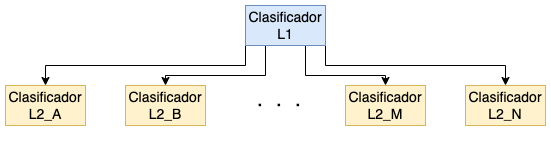
\includegraphics[width=.8\textwidth]{./Figures/cap3-redes.png}
	\caption{Diagrama general de los modelos de IA.}
	\label{fig:cap3-redes}
\end{figure}

Este diseño presenta una serie de ventajas, entre las que principalmente se destaca su diseño modular. Esto es importante para la etapa de soporte a futuro, ya que si surge una nueva categoría o se quiere mejorar una parte de la clasificación, sólo es necesario trabajar en el modelo afectado dejando los demás intactos.

Además, al hacer que cada clasificador tenga que realizar una tarea más específica, su \textit{head} de clasificación también queda más simple.

\subsection{Entrenamiento de los modelos base}

Un modelo base o \textit{baseline} es un modelo simple que actúa como referencia y sirve para tener con qué comparar cuando se entrenan modelos más complejos. 

Las ventajas de utilizar un modelo base son las siguientes \citep{WEBSITE:23}:
\begin{itemize}
	\item Se entrenan rápidamente y sin recursos especializados.
	\item Permite tener un mejor entendimiento en etapas tempranas.
	\item Sirven para encontrar errores y poner a prueba suposiciones.
	\item Sirven para medir el progreso de los modelos más complejos.
\end{itemize}

Como se mencionó en el capítulo \ref{Chapter2}, para este trabajo el \textit{baseline} elegido fue CNB de la librería Scikit-Learn. La clase provista se llama \textit{ComplementNB} y provee un método \textit{fit} para realizar el entrenamiento y un método \textit{predict} para realizar una predicción sobre datos que se pasan como parámetro.

El entorno donde se realizó el entrenamiento fue una computadora local.

\subsubsection{Modelos base en validación cruzada}

Hubo algunas categorías en particular que cuando se quiso entrenar el clasificador L2, contaban con muy pocos datos incluso tomando del año 2023. Estas categorías fueron:
\begin{itemize}
	\item L2\_L.
	\item L2\_N.
\end{itemize}

La primera contaba con un total de 200 casos y cuando se incluyeron los de 2023  se llegó a tener 267. Para este caso, lo que se hizo fue obtener una métrica en validación cruzada usando la clase RepeatedStratifiedKFold de Scikit-Learn con 5 \textit{folds} y 5 repeats. Luego se procedió a entrenar el modelo CNB final utilizando el set de datos completo.

La segunda contaba originalmente con sólo 2 casos y cuando se incluyeron los de 2023 se llegó a 8. Este resultó ser un caso muy extremo, donde se utilizó otra técnica de validación cruzada con la clase LeaveOneOut de Scikit-Learn. Lo que hace esta técnica es ir apartando un dato por \textit{fold} y entrenar con el resto. Una vez tomada la métrica, se entrenó el CNB final con todos los datos.

\subsection{Entrenamiento de BERT}

Como los textos del \textit{dataset} estaban escritos en español, se utilizó la red BETO. Este modelo es un modelo BERT entrenado con el dataset \textit{spanish unannotated corpora} que cuenta con casi tres millardos de palabras. Está disponible dentro de la librería Transformers de HuggingFace para Python, tanto en Pytorch como en Tensorflow. Para este trabajo se utilizó esta última.

Por otro lado, estos modelos pre-entrenados deben ser adaptados para realizar tareas como clasificación de texto. En la figura \ref{fig:cap3-downstream} se muestra un esquema de entrenamiento de BETO.

\begin{figure}[htbp]
	\centering
	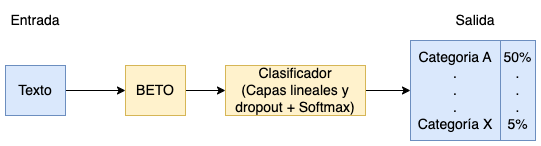
\includegraphics[width=.9\textwidth]{./Figures/cap3-downstream.png}
	\caption{Esquema de entrenamiento de BERT para clasificación de texto.}
	\label{fig:cap3-downstream}
\end{figure}

Se puede notar que sobre el modelo pre-entrenado de BETO se agrega: un \textit{head} de clasificación compuesto por perceptrones multicapa combinados con técnicas de regularización como \textit{dropout} y por último \textit{softmax} como función de activación para realizar la tarea de clasificación per se.

\subsubsection{Aprendizaje por transferencia}

El aprendizaje por transferencia consiste en entrenar un modelo en un conjunto de datos (por lo general a gran escala) y luego usar ese modelo previamente entrenado para llevar a cabo el aprendizaje para otra tarea posterior (la tarea objetivo) \citep{WEBSITE:24}.

Se distinguen tres métodos para transferir el aprendizaje:
\begin{itemize}
	\item Extracción de características: se usan las capas pre-entrenadas para extraer características o \textit{features} de los datos. Los pesos de las capas inferiores no se actualizan durante el \textit{backpropagation}.
	\item Ajuste fino: se ajustan todos los parámetros del modelo.
	\item Extracción de capas: se extraen sólo las capas necesarias para la tarea en cuestión.
\end{itemize}

Para este trabajo, el aprendizaje por transferencia consistió en utilizar el modelo pre-entrenado de BETO y luego ajustarlo para la tarea de clasificación de reclamos.

En primera instancia se utilizó el método de extracción de características que consistió en congelar las capas de BETO y dejar libre el \textit{head} de clasificación para entrenar sus pesos. Para esto, se dejó el \textit{learning rate} default de Tensorflow.

[FIGURA CANDADITO]

Luego, se realizó un ajuste fino, dejando libres todas las capas del modelo para ajustar todos sus pesos, esta vez con un \textit{learning rate} más bajo.

[FIGURA SIN CANDADITO]

La técnica de extracción de capas no fue utilizada en este trabajo.

\subsubsection{Entorno de entrenamiento}



\subsubsection{Puntos de control y parada temprana}



\subsubsection{Efecto de usar \textit{stopwords} en el entrenamiento}

\subsubsection{Técnicas para el desbalanceo de clases}

\subsubsection{Optimizadores}


\section{Desarrollo de GitHub Actions}



\section{Empaquetamiento del código y artefactos}



\section{Desarrollo del \textit{pipeline} de predicción}



\section{Almacenamiento de predicciones}


% Chapter Template

\chapter{Ensayos y resultados} % Main chapter title

\label{Chapter4} % Change X to a consecutive number; for referencing this chapter elsewhere, use \ref{ChapterX}

En este capítulo se presenta y describe la métrica elegida para evaluar el desempeño de los modelos entrenados, se muestran los resultados obtenidos y por último, se explican las simulaciones realizadas en un ambiente de desarrollo para probar la ejecución del flujo de trabajo de Airflow.

\section{Métrica de evaluación de los modelos}

Para evaluar un sistema de clasificación automático, en general se suele usar una matriz de confusión. Esta matriz es una tabla de doble entrada, donde cada columna muestra el número de predicciones de cada clase y cada fila muestra el número real de instancias de cada clase. En la figura \ref{fig:matriz-confusion} puede observarse una para clasificación multiclase:

\begin{figure}[htbp]
	\centering
	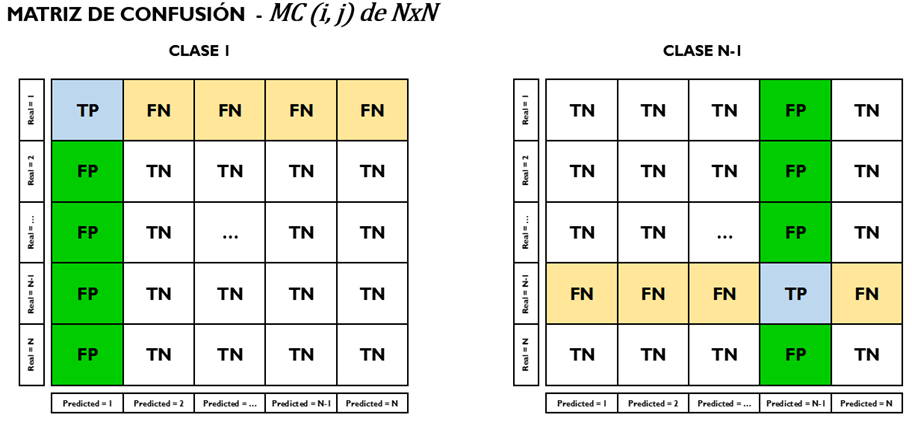
\includegraphics[width=1\textwidth]{./Figures/matriz-confusion.png}
	\caption{Ejemplo de matriz de confusión multiclase genérica\protect\footnotemark.}
	\label{fig:matriz-confusion}
\end{figure}

\footnotetext{Imagen tomada de \url{https://wbarriosb.medium.com/calculando-la-precisi\%C3\%B3n-en-un-modelo-de-clasificaci\%C3\%B3n-multiclase-224d96f52043}}

Para entender esta matriz, es necesario presentar cuatro conceptos que vienen asociados:
\begin{itemize}
	\item Verdaderos positivo (VP o TP): la cantidad de positivos clasificados como positivos por el modelo.
	\item Falso negativo (FN): la cantidad de positivos clasificados como negativos por el modelo.
	\item Verdadero negativo (VN o TN): la cantidad de negativos clasificados como negativos por el modelo.
	\item Falso positivo (FP): la cantidad de negativos clasificados como positivos por el modelo.
\end{itemize}

Presentar los resultados en esta matriz permite calcular distintas métricas para evaluar características del sistema de clasificación. Por ejemplo:

La precisión, que está relacionada con la capacidad del modelo de no predecir un positivo cuando en realidad es un negativo:
\begin{equation}
\text{precisión}_{k}=\frac{MC(k,k)}{\sum_{i=1,j=k}^{N}MC(i,j)}
\end{equation}

La exhaustividad, que está relacionada con la capacidad del modelo de detectar todos los positivos:
\begin{equation}
\text{exhaustividad}_{k}=\frac{MC(k,k)}{\sum_{j=1,i=k}^{N}MC(i,j)}
\end{equation}

Para este trabajo, la métrica seleccionada para evaluar el desempeño de los modelos fue el puntaje F1 o \textit{F1-Score}. Lo que hace esta métrica es calcular la media armónica entre la precisión y la exhaustividad \textit{(recall)} del modelo. Su fórmula es la siguiente:
\begin{equation}
\text{F1}_{k}=2\times \frac{\text{precisión}_{k}\times \text{exhaustividad}_{k}}{\text{precisión}_{k}+ \text{exhaustividad}_{k}}
\end{equation}

De esta forma, se estaría obteniendo el F1 para cada clase. Para calcular un F1 global del sistema de clasificación, existen tres tipos de estrategia \citep{WEBSITE:28}
\begin{itemize}
	\item \textit{Macro average}: consiste en calcular la media aritmética de todos los F1 calculados para cada clase. Esta estrategia le da a todas las clases la misma importancia en el cálculo del F1 global.
	\item \textit{Micro average}: consiste en calcular el F1 considerando el número total de TP, FP y FN, en lugar de hacerlo por cada clase. Esta estrategia calcula la proporción de las observaciones clasificadas correctamente sobre las observaciones totales.
	\item \textit{Weighted average}: consiste en calcular la media aritmética de todos los F1 calculados para cada clase, pero ponderando el soporte de cada clase (la cantidad de observaciones). Esta estrategia le da más importancia a las clases con más observaciones para el cálculo del F1 global.
\end{itemize}

Para \textit{datasets} balanceados, es decir, cuando tienen una cantidad de observaciones parecida para cada una de las clases, se suele usar el \textit{micro average}. No es el caso de este trabajo, donde por la naturaleza de los reclamos, hubo categorías que presentaron más observaciones que otras.

Dentro de las dos opciones restantes, se decidió por utilizar el \textit{weighted} F1, ya que para medir el desempeño del modelo, se pretende dar una mayor importancia a las clases cuyos reclamos aparecen más a menudo. 

La fórmula se muestra a continuación:
\begin{equation}
\text{F1}_{global}=\sum_{k=1}^{N}\text{F1}_{k} \times \text{soporte}_{k} 
\end{equation}

\section{Resultados de desempeño en pruebas}

En esta sección se presentan los resultados obtenidos para todos los modelos entrenados de cada categoría.

\subsection{Resultados para clasificador L1}

En la figura \ref{fig:res-l1} se pueden observar los distintos entrenamientos realizados para el clasificador L1 y su puntaje obtenido.

\begin{figure}[htbp]
	\centering
	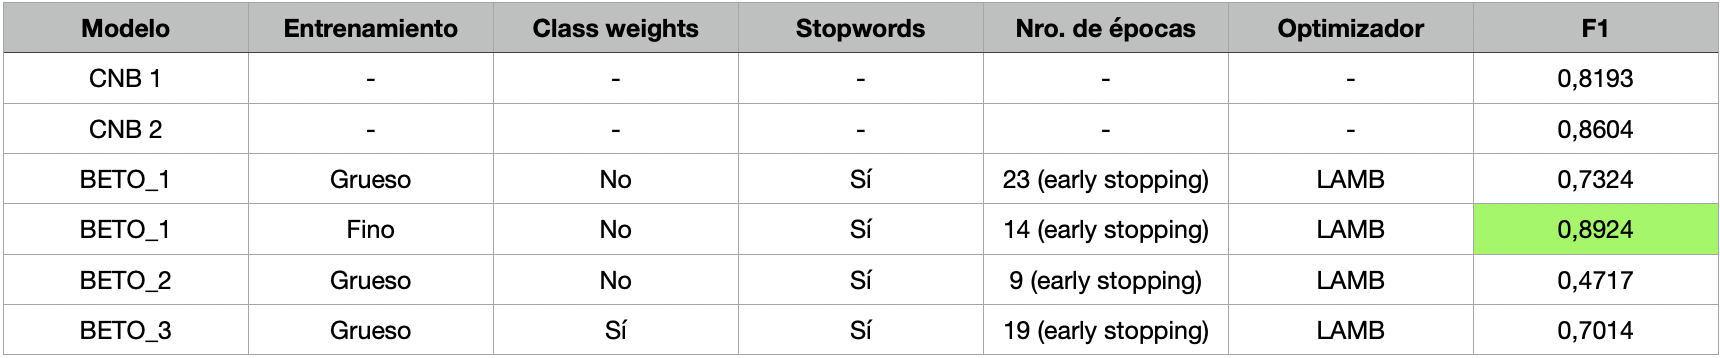
\includegraphics[width=1\textwidth]{./Figures/cap4-resultados-l1.png}
	\caption{Resultados obtenidos para los modelos clasificadores L1.}
	\label{fig:res-l1}
\end{figure}

A continuación se hacen algunas aclaraciones respecto de los modelos:
\begin{itemize}
	\item Modelo CNB\_1: los reclamos pertenecientes a la categoría especial que se menciona en la subsección \ref{sec:extraccion} fueron eliminados.
	\item Modelo CNB\_2: los reclamos pertenecientes a la categoría especial fueron redireccionados a otras categorías L1.
	\item Modelo BETO\_1: los reclamos pertenecientes a la categoría especial fueron eliminados.
	\item Modelo BETO\_2: los reclamos pertenecientes a la categoría especial fueron redireccionados a otras categorías L1.
	\item Modelo BETO\_3: los reclamos pertenecientes a la categoría especial fueron eliminados.
\end{itemize}

\subsection{Resultados para clasificador L2 A}

En la figura \ref{fig:res-l2a} se pueden observar los distintos entrenamientos realizados para el clasificador L2 A y su puntaje obtenido.

\begin{figure}[H]
	\centering
	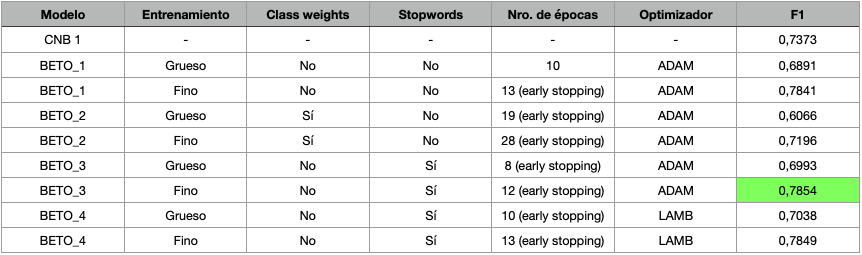
\includegraphics[width=1\textwidth]{./Figures/cap4-resultados-l2a.png}
	\caption{Resultados obtenidos para los modelos clasificadores L2 A.}
	\label{fig:res-l2a}
\end{figure}

Aclaración: el modelo BETO\_4 cuenta con un \textit{head} de clasificación de dos capas.

\subsection{Resultados para clasificador L2 B}

En la figura \ref{fig:res-l2b} se muestran los entrenamientos realizados para el clasificador L2 B y sus resultados.

\begin{figure}[htbp]
	\centering
	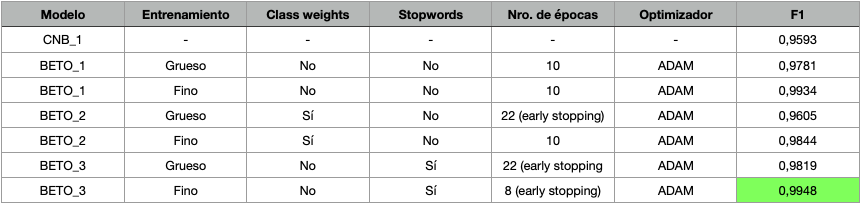
\includegraphics[width=1\textwidth]{./Figures/cap4-resultados-l2b.png}
	\caption{Resultados obtenidos para los modelos clasificadores L2 B.}
	\label{fig:res-l2b}
\end{figure}

\subsection{Resultados para clasificador L2 C}

En la figura \ref{fig:res-l2c} se presentan los resultados para los entrenamientos del clasificador L2 C.

\begin{figure}[H]
	\centering
	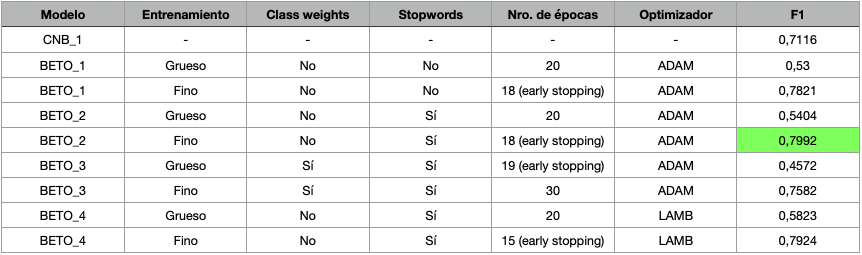
\includegraphics[width=1\textwidth]{./Figures/cap4-resultados-l2c.png}
	\caption{Resultados obtenidos para los modelos clasificadores L2 C.}
	\label{fig:res-l2c}
\end{figure}

Aclaración: los modelos entrenados con LAMB cuentan con un \textit{head} de clasificación de dos capas.

\subsection{Resultados para clasificador L2 D}

A continuación se muestra la figura \ref{fig:res-l2d} con los resultados para los entrenamientos del clasificador L2 D.

\begin{figure}[htbp]
	\centering
	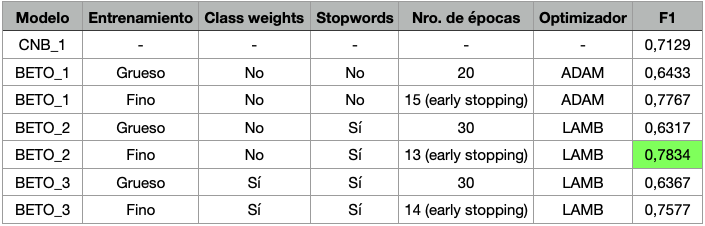
\includegraphics[width=1\textwidth]{./Figures/cap4-resultados-l2d.png}
	\caption{Resultados obtenidos para los modelos clasificadores L2 D.}
	\label{fig:res-l2d}
\end{figure}

Aclaración: los modelos entrenados con LAMB cuentan con un \textit{head} de clasificación de dos capas.

\subsection{Resultados para clasificador L2 E}

En la figura \ref{fig:res-l2e} se pueden observar los distintos entrenamientos realizados para el clasificador L2 E y su puntaje obtenido.

\begin{figure}[H]
	\centering
	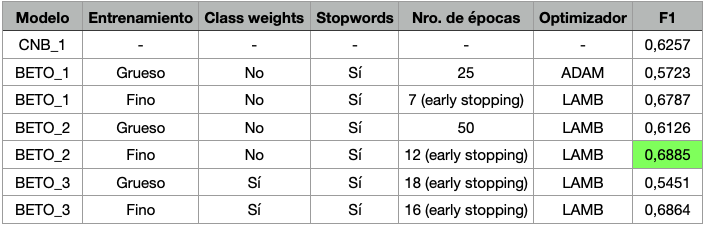
\includegraphics[width=1\textwidth]{./Figures/cap4-resultados-l2e.png}
	\caption{Resultados obtenidos para los modelos clasificadores L2 E.}
	\label{fig:res-l2e}
\end{figure}

A continuación se hacen algunas aclaraciones:
\begin{itemize}
	\item Los modelos CNB\_1 y BETO\_1 fueron entrenados únicamente con el dataset que tenía datos hasta 2022. Algunas categorías no tenían datos hasta esa fecha, por lo que los modelos fueron entrenados con datos faltantes para esas categorías.
	\item Los modelos BETO\_2 y BETO\_3 fueron entrenados con el dataset que tenía datos hasta 2022 pero incluyendo datos de 2023 para las categorías que no tenían datos.
\end{itemize}

\subsection{Resultados para clasificador L2 F}

En la figura \ref{fig:res-l2f} se muestran los entrenamientos realizados para el clasificador L2 F y sus resultados.

\begin{figure}[H]
	\centering
	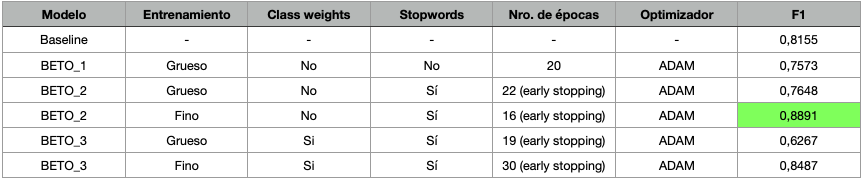
\includegraphics[width=1\textwidth]{./Figures/cap4-resultados-l2f.png}
	\caption{Resultados obtenidos para los modelos clasificadores L2 F.}
	\label{fig:res-l2f}
\end{figure}

\subsection{Resultados para clasificador L2 G}

En la figura \ref{fig:res-l2g} se presentan los resultados para los entrenamientos del clasificador L2 G.

\begin{figure}[htbp]
	\centering
	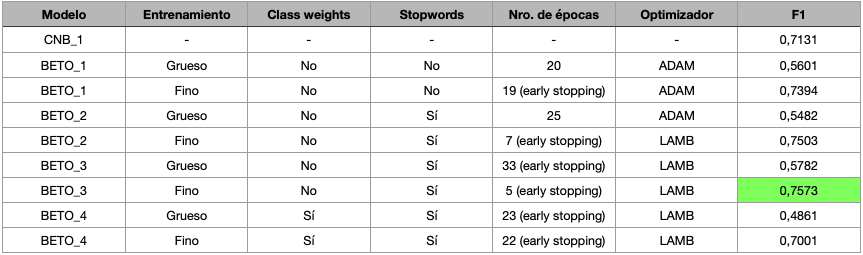
\includegraphics[width=1\textwidth]{./Figures/cap4-resultados-l2g.png}
	\caption{Resultados obtenidos para los modelos clasificadores L2 G.}
	\label{fig:res-l2g}
\end{figure}

Aclaración: los modelos BETO\_3 y BETO\_4 fueron entrenados con un \textit{head} de clasificación de dos capas.

\subsection{Resultados para clasificador L2 H}

A continuación se muestra la figura \ref{fig:res-l2h} con los resultados para los entrenamientos del clasificador L2 H.

\begin{figure}[htbp]
	\centering
	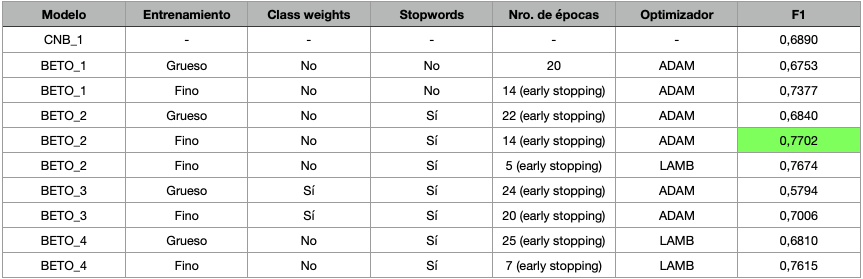
\includegraphics[width=1\textwidth]{./Figures/cap4-resultados-l2h.png}
	\caption{Resultados obtenidos para los modelos clasificadores L2 H.}
	\label{fig:res-l2h}
\end{figure}

Aclaración: el modelo BETO\_4 fue entrenado con un \textit{head} de clasificación de dos capas.

\subsection{Resultados para clasificador L2 I}

En la figura \ref{fig:res-l2i} se presentan los resultados para los entrenamientos del clasificador L2 I.

\begin{figure}[htbp]
	\centering
	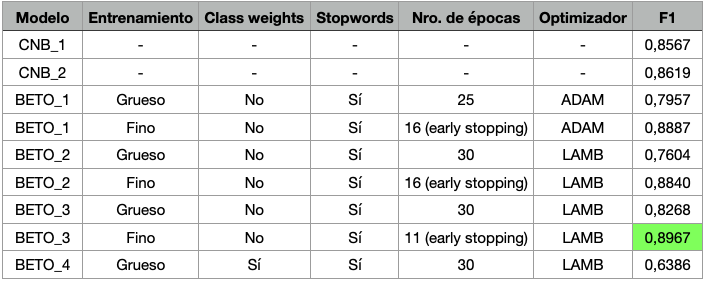
\includegraphics[width=1\textwidth]{./Figures/cap4-resultados-l2i.png}
	\caption{Resultados obtenidos para los modelos clasificadores L2 I.}
	\label{fig:res-l2i}
\end{figure}

Se hacen algunas aclaraciones:
\begin{itemize}
	\item Tanto el dataset que tenía datos hasta 2022 como el que incluía datos de 2023 carecían de datos para algunas categorías.
	\item Todos los modelos entrenados con LAMB contaban con un \textit{head} de clasificación de dos capas.
	\item El modelo BETO\_1 fue entrenado exclusivamente con el dataset original.
	\item El modelo BETO\_2 fue entrenado con el dataset original y se incluyeron datos de 2023 para las categorías sin datos.
	\item Los modelos BETO\_3 y BETO\_4 fueron entrenados con datos hasta 2023 inclusive para todas las categorías.
\end{itemize}

\subsection{Resultados para clasificador L2 J}

A continuación se muestra la figura \ref{fig:res-l2j} con los resultados para los entrenamientos del clasificador L2 J.

\begin{figure}[htbp]
	\centering
	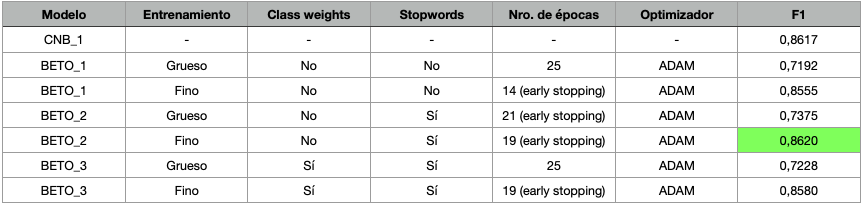
\includegraphics[width=1\textwidth]{./Figures/cap4-resultados-l2j.png}
	\caption{Resultados obtenidos para los modelos clasificadores L2 J.}
	\label{fig:res-l2j}
\end{figure}

\subsection{Resultados para clasificador L2 K}

En la figura \ref{fig:res-l2k} se presentan los resultados para los entrenamientos del clasificador L2 K.

\begin{figure}[htbp]
	\centering
	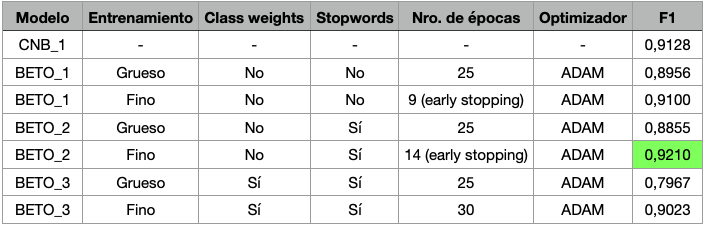
\includegraphics[width=1\textwidth]{./Figures/cap4-resultados-l2k.png}
	\caption{Resultados obtenidos para los modelos clasificadores L2 K.}
	\label{fig:res-l2k}
\end{figure}

\subsection{Resultados para clasificador L2 L}

En la figura \ref{fig:res-l2l} se presentan los resultados para los entrenamientos del clasificador L2 L.

\begin{figure}[htbp]
	\centering
	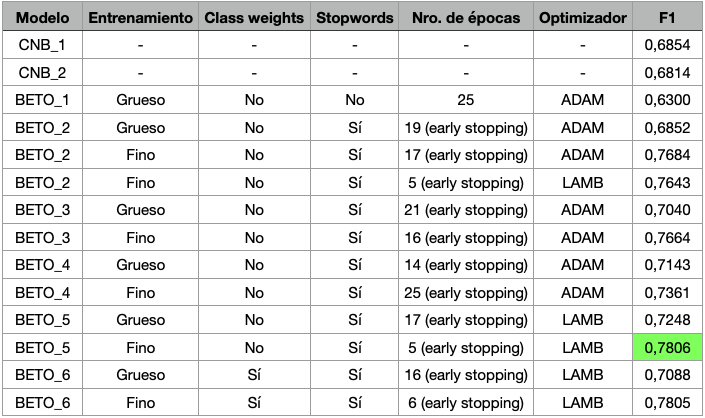
\includegraphics[width=1\textwidth]{./Figures/cap4-resultados-l2l.png}
	\caption{Resultados obtenidos para los modelos clasificadores L2 L.}
	\label{fig:res-l2l}
\end{figure}

Se hacen algunas aclaraciones de los modelos:
\begin{itemize}
	\item Los modelos CNB\_1, BETO\_1 y BETO\_2 fueron entrenados con el dataset original que tenía datos hasta 2022 inclusive.
	\item Los modelos CNB\_2, BETO\_3, BETO\_5 y BETO\_6 fueron entrenados con el dataset que también incluía datos de 2023.
	\item Para el entrenamiento del modelo BETO\_4 se utilizó el dataset original que tenía datos hasta 2022 y además se incluyeron datos de 2023 para la clase minoritaria.
	\item Para los modelos BETO\_5 y BETO\_6 se utilizó un \textit{head} de clasificación de dos capas.
\end{itemize}

\subsection{Resultados para clasificador L2 M}

Como se mencionó en la sección \ref{sec:kfolds}, el entrenamiento del modelo L2 M fue particular porque se contaban con 267 muestras incluyendo los casos de 2023. Se decidió obtener una métrica con validación cruzada para tener una medida de desempeño y luego entrenar un modelo con todos los datos. En este caso el F1 obtenido fue 0,5568.

\subsection{Resultados para clasificador L2 N}

Además, en la sección \ref{sec:kfolds} también se hace mención al modelo L2 N, que fue un caso extremo donde sólo había 8 muestras incluyendo los datos de 2023. Aquí se utilizó la técnica de \textit{leave one out} y el F1 obtenido fue 0,7500.

\section{Simulación en ambiente de desarrollo}

Las pruebas realizadas en la nube de Google incluyeron el despliegue de la solución en un ambiente de desarrollo con recursos similares a los de un ambiente de producción, pero con menor capacidad de cómputo.

La infraestructura utilizada de Google fue:
\begin{itemize}
	\item Cloud Storage: se creó un contenedor para el almacenamiento de los archivos de los modelos.
	\item Artifact Registry: se cargó la imagen de Docker al registro correspondiente al ambiente de desarrollo.
	\item Cloud Composer/Airflow: se sincronizó el código del DAG al Composer del ambiente de desarrollo.
	\item BigQuery: se utilizaron los datasets correspondientes al ambiente de desarrollo para el almacenamiento de las tablas con los resultados.
	\item Kubernetes Engine: se utilizó el clúster de Kubernetes en modo \textit{autopilot} del ambiente de desarrollo.
\end{itemize}

En la figura \ref{fig:cap4-dag} se pueden ver las ejecuciones del DAG en Airflow.

\begin{figure}[htbp]
	\centering
	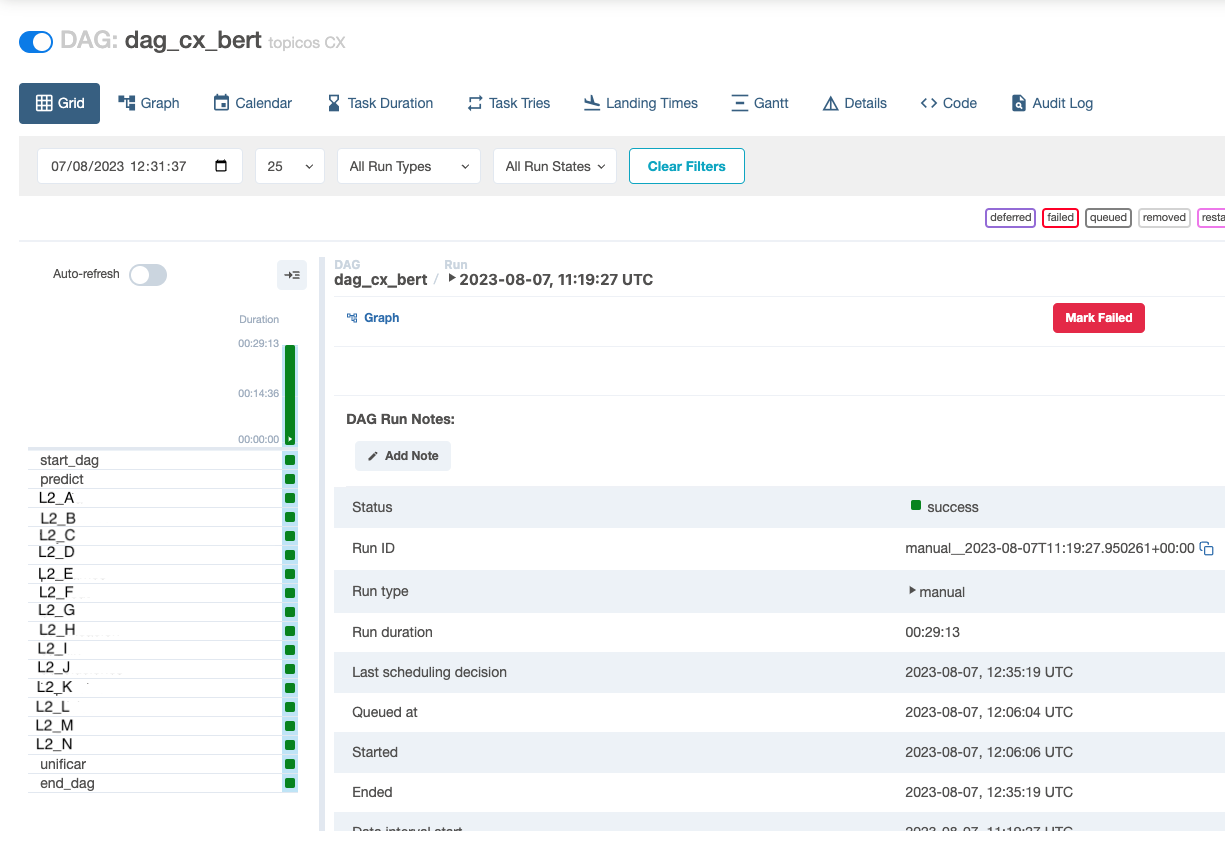
\includegraphics[width=1\textwidth]{./Figures/cap4-dag.png}
	\caption{Ejecución de un DAG en Airflow.}
	\label{fig:cap4-dag}
\end{figure}

Al estar en un ambiente de desarrollo, la disponibilidad de los recursos fue limitada. Se configuró Airflow para que la ejecución de los operadores del DAG fuera secuencial, es decir, de a uno por vez. En promedio, la ejecución total del DAG tomó 30 minutos. Estos tiempos se podrían mejorar paralelizando la ejecución de los operadores que predicen las categorías L2. Igualmente, esto no supone un problema para la solución, ya que la predicción se hace en forma \textit{batch} y no en tiempo real.

En la tabla \ref{tab:gke} se pueden ver los recursos utilizados para cada paso de predicción del DAG.
\begin{table}[h]
	\centering
	\caption[Especificaciones técnicas Pod]{Especificaciones técnicas del Pod para predicción.}
	\begin{tabular}{l c}    
		\toprule
		\textbf{Componente}			& 			\textbf{Descripción}  \\
		\midrule	
		Nro. de núcleos virtuales	& 			8 vCPUs  \\
		Memoria RAM					&			8 GB \\
		Nro. de placas de video 	& 			1  \\
		Versión de placa de video	&			Nvidia T4 \\
		Memoria de placa de video	& 			16 GB GDDR6  \\
		\bottomrule
		\hline
	\end{tabular}
	\label{tab:gke}
\end{table}

En la figura \ref{fig:cap4-pod} se muestra la ejecución de un Pod en el Kubernetes Engine:

\begin{figure}[htbp]
	\centering
	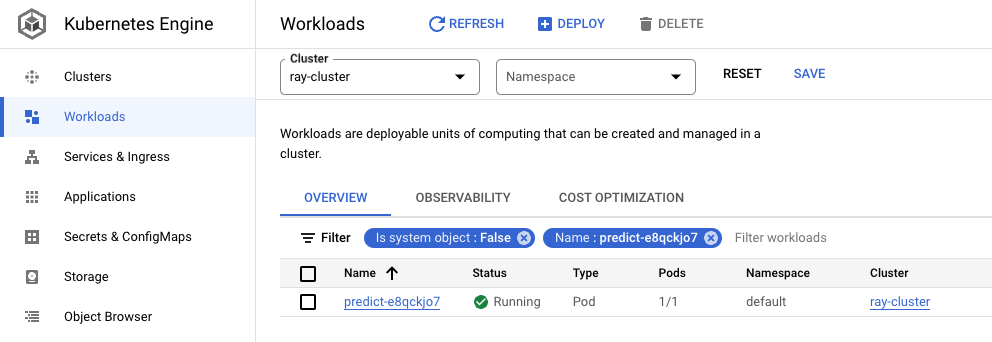
\includegraphics[width=1\textwidth]{./Figures/cap4-pod.png}
	\caption{Ejecución de un Pod en el Kubernetes Engine.}
	\label{fig:cap4-pod}
\end{figure}

La imagen que se carga en el contenedor del Pod se descarga desde el Artifact Registry, como se ve en la figura \ref{fig:cap4-ar}:

\begin{figure}[H]
	\centering
	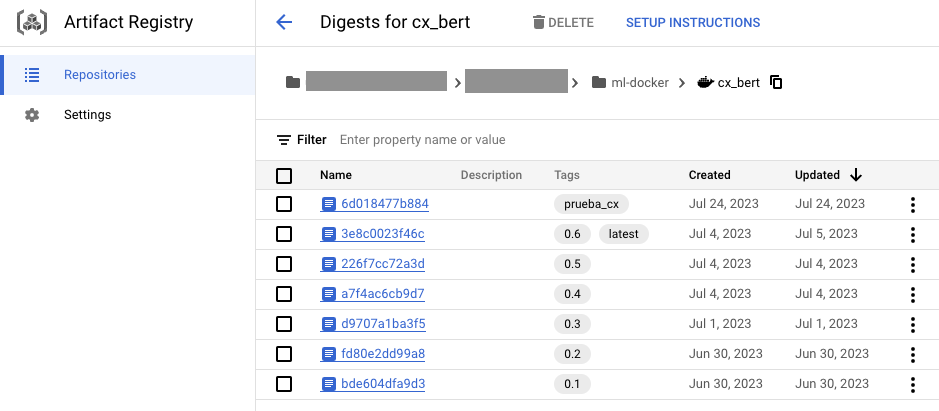
\includegraphics[width=1\textwidth]{./Figures/cap4-ar.png}
	\caption{Imágenes de Docker en el Artifact Registry.}
	\label{fig:cap4-ar}
\end{figure}

Por otro lado, en la figura \ref{fig:cap4-bq} se puede ver la estructura de la tabla que contiene los resultados de una predicción:

\begin{figure}[htbp]
	\centering
	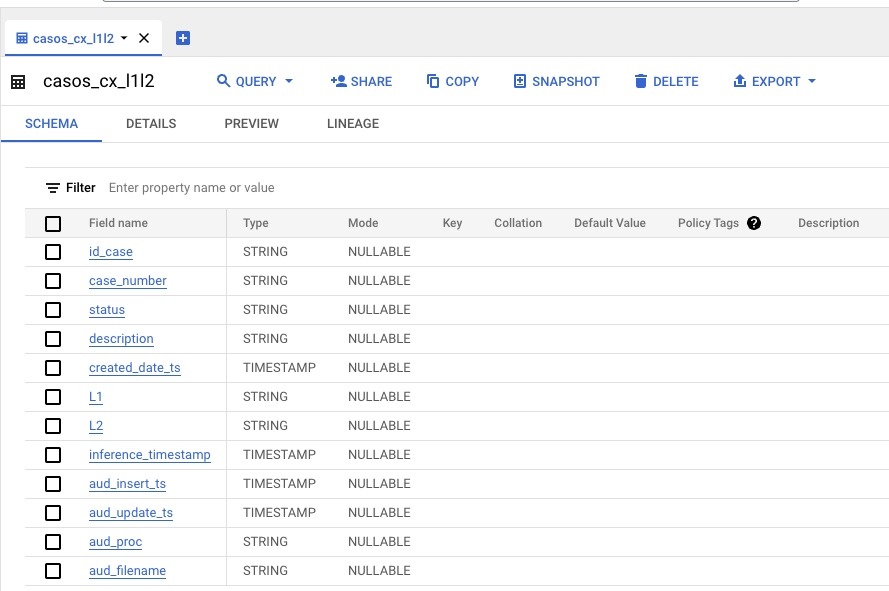
\includegraphics[width=1\textwidth]{./Figures/cap4-bq.png}
	\caption{Estructura de la tabla de resultados en BigQuery.}
	\label{fig:cap4-bq}
\end{figure}

 
% Chapter Template

\chapter{Conclusiones} % Main chapter title

\label{Chapter5} % Change X to a consecutive number; for referencing this chapter elsewhere, use \ref{ChapterX}

En este capítulo se presentan los resultados del trabajo y posibles mejoras a futuro.

\section{Conclusiones generales}

Se desarrolló un sistema de clasificación de reclamos de manera exitosa, incluyendo su despliegue en un ambiente de desarrollo, cumpliendo con todos los requerimientos funcionales y no funcionales. Se pudo cumplir con la planificación original y finalizar el total de las tareas, a pesar de que las actividades relacionadas al entrenamiento de los modelos llevaron más horas de las asignadas inicialmente.

A continuación se listan los logros del trabajo final:
\begin{itemize}
	\item Identificar la categoría principal de los reclamos con un F1 de 0,8924.
	\item Identificar la subcategoría de los reclamos con un F1 superior a 0,77 excepto para dos clasificadores.
	\item Haber desplegado un proceso de predicción en un ambiente de desarrollo, utilizando la infraestructura y herramientas que el área dispuso.
\end{itemize}

A continuación, se destacan las materias de la carrera de mayor relevancia para la realización de este trabajo:
\begin{itemize}
	\item Procesamiento del lenguaje natural: fue extremadamente importante para aplicar técnicas de preprocesamiento de texto, vectorización y clasificación de texto.
	\item Bases de datos: para poder realizar la extracción de los datos y para almacenar los resultados.
	\item Gestión de proyectos: para elaborar un plan y bajarlo a un calendario específico, que posibilitó cumplir con los plazos estipulados.
\end{itemize}


\section{Próximos pasos}

Luego de haber finalizado este trabajo, se identifican dos tipos de mejoras posibles: 
\begin{itemize}
	\item De desempeño.
	\item De funcionalidad.
\end{itemize}

Una alternativa para mejorar el desempeño de los clasificadores puede ser probar modelos de IA más avanzados y con mayor cantidad de parámetros, como la versión \textit{large} de BERT o incluso probando ROBERTA, que requieren un poder mayor de cómputo que el utilizado. Esto puede resultar particularmente importante para el clasificador L2\_E cuya métrica F1 resultó inferior a 0,7, y también para el clasificador L1 por su impacto en la clasificación final de las subcategorías.

En cuanto a la funcionalidad, durante el transcurso de este trabajo, la empresa ha lanzado nuevos productos que involucran nuevas categorías de reclamos. Cuando se tenga un dataset de tamaño significativo, se puede re-entrenar el clasificador L1 para incluir las nuevas categorías y los clasificadores L2 para las subcategorías correspondientes.

Por otro lado, se pueden entrenar nuevos clasificadores para las categorías L3 más importantes, y de esta forma, cubrir el árbol de clasificación completo del proceso de atención de reclamos y consultas de la empresa.
 

%----------------------------------------------------------------------------------------
%	CONTENIDO DE LA MEMORIA  - APÉNDICES
%----------------------------------------------------------------------------------------

\appendix % indicativo para indicarle a LaTeX los siguientes "capítulos" son apéndices

% Incluir los apéndices de la memoria como archivos separadas desde la carpeta Appendices
% Descomentar las líneas a medida que se escriben los apéndices

%\include{Appendices/AppendixA}
%\include{Appendices/AppendixB}
%\include{Appendices/AppendixC}

%----------------------------------------------------------------------------------------
%	BIBLIOGRAPHY
%----------------------------------------------------------------------------------------

\Urlmuskip=0mu plus 1mu\relax
\raggedright
\printbibliography[heading=bibintoc]

%----------------------------------------------------------------------------------------

\end{document}  
